%%%%%%%%%%%%%%%%%%%%%%%%%%%%%%%%%%%%%%%%%%%%%%%%%%%%%%%%%%%%%%%%%%%%%%%%%%%%%%%%
%2345678901234567890123456789012345678901234567890123456789012345678901234567890
%        1         2         3         4         5         6         7         8

\documentclass[journal,transmag]{IEEEtran}% Comment this line out if you need a4paper

%\documentclass[a4paper, 10pt, conference]{ieeeconf}      % Use this line for a4 paper

\IEEEoverridecommandlockouts                              % This command is only needed if 
                                                          % you want to use the \thanks command

%\overrideIEEEmargins                                      % Needed to meet printer requirements.

% See the \addtolength command later in the file to balance the column lengths
% on the last page of the document

% The following packages can be found on http:\\www.ctan.org
%\usepackage{graphics} % for pdf, bitmapped graphics files
%\usepackage{epsfig} % for postscript graphics files
%\usepackage{mathptmx} % assumes new font selection scheme installed
%\usepackage{times} % assumes new font selection scheme installed
%\usepackage{amsmath} % assumes amsmath package installed
%\usepackage{amssymb}  % assumes amsmath package installed



\usepackage{amsmath,amssymb}

\usepackage{tikz,hyperref,graphicx,units,subfig}
\usepackage{subfig}
\usepackage{benktools}
\usepackage{caption}
\renewcommand{\captionfont}{\footnotesize}
\usepackage{sidecap,wrapfig}
\usepackage[ruled,vlined]{algorithm2e}
\DeclareMathOperator*{\argmin}{arg\,min}
\DeclareMathOperator*{\argmax}{arg\,max}
\newcommand{\abs}[1]{\lvert#1\rvert} 
\newcommand{\norm}[1]{\lVert#1\rVert}
%\newcommand{\suchthat}{\mid}
\newcommand{\suchthat}{\ \big|\ }
\newcommand{\ba}{\mathbf{a}}
\newcommand{\bb}{\mathbf{b}}
\newcommand{\bc}{\mathbf{c}}
\newcommand{\bd}{\mathbf{d}}
\newcommand{\bn}{\mathbf{n}}
\newcommand{\bp}{\mathbf{p}}
\newcommand{\bw}{\mathbf{w}}
\newcommand{\bt}{\mathbf{t}}
\newcommand{\by}{\mathbf{y}}
\newcommand{\bx}{\mathbf{x}}
\newcommand{\bz}{\mathbf{z}}
\newcommand{\bbf}{\mathbf{f}}
\newcommand{\bzero}{\mathbf{0}}
\newcommand{\bG}{\mathbf{G}}
\newcommand{\bA}{\mathbf{A}}
\newcommand{\bW}{\mathbf{W}}
\newcommand{\bX}{\mathbf{X}}
\newcommand{\mX}{\mathcal{X}}
\newcommand{\mD}{\mathcal{D}}
\newcommand{\mG}{\mathcal{G}}
\newcommand{\mN}{\mathcal{N}}
\newcommand{\mW}{\mathcal{W}}
\newcommand{\mF}{\mathcal{F}}
\newcommand{\bZ}{\mathbf{Z}}

\newcommand{\bfc}{W}
\newcommand{\Qinf}{Q_{\infty}}
\newcommand{\st}[1]{_\text{#1}}
\newcommand{\rres}{r\st{res}}
\newcommand{\pos}[1]{(#1)^+}
\newcommand{\depth}{\operatorname{depth}}
\newcommand{\dist}{\operatorname{dist}}
\newcommand{\convhull}{\operatorname{ConvexHull}}
\newcommand{\minksum}{\operatorname{MinkowskiSum}}

\title{\LARGE \bf
Efficient Planar Sample-Based Grasp Planning with Uncertainty Using Budgeted Multi-Armed Bandit Models for  [v3 Jan 5, 2015 ] }


\author{Michael Laskey$^1$,Jeff Mahler$^1$, Zoe McCarthy$^1$,  Florian T. Pokorny$^3$, Sachin Patil$^1$,\\ Jur Van Den Berg$^4$,  Danica Kragic$^3$, Pieter Abbeel$^1$, Ken Goldberg$^2$% <-this % stops a space
\thanks{$^1$Department of Electrical Engineering and Computer Sciences; {\small \{mdlaskey, zmccarthy, jmahler, sachinpatil, pabbeel\}@berkeley.edu}}%
\thanks{$^2$Department of Industrial Engineering and Operations Research and Department of Electrical Engineering and Computer Sciences; {\small goldberg@berkeley.edu}}%
\thanks{$^{1-2}$ University of California, Berkeley;  Berkeley, CA 94720, USA}%
\thanks{$^3$Computer Vision and Active Perception Lab, Centre for Autonomous Systems, School of Computer Science and Communication, KTH Royal Institute of Technology, Stockholm, Sweden {\small \{fpokorny, dani\}@kth.se}}%
\thanks{$^4$Google; Amphitheatre Parkway, Mountain View, CA 94043, USA {\small jurvandenberg@gmail.com}}%
} 

\newtheorem{theorem}{Theorem}

\begin{document}



\maketitle
\thispagestyle{empty}
\pagestyle{empty}


%%%%%%%%%%%%%%%%%%%%%%%%%%%%%%%%%%%%%%%%%%%%%%%%%%%%%%%%%%%%%%%%%%%%%%%%%%%%%%%%

\begin{abstract}
\textit{Abstract---}\todo{Not sure if we need to change the authors list or not}Sampling perturbations in shape, state, and control can facilitate grasp planning in the presence of uncertainty arising from noise, occlusions, and surface properties such as transparency and specularities.  Monte-Carlo sampling is computationally demanding, even for planar models. We consider an alternative based on the multi-armed bandit (MAB) model for making sequential decisions, which can apply to a variety of uncertainty models.  We formulate grasp planning as a ``budgeted multi-armed bandit model" (BMAB) with finite stopping time to minimize ``simple regret", the difference between the expected quality of the best grasp and the expected quality of the grasp evaluated at the stopping time.  To evaluate MAB-based sampling, we compare it with Monte-Carlo sampling for grasping an uncertain planar object with shape uncertainty defined by a Gaussian process implicit surface (GPIS), but the method is also applicable to other models of uncertainty.  We derive distributions on contact points, surface normal, and center of mass under shape uncertainty and use these to formulate the associated MAB model, finding that it computes grasps of similar quality to Monte-Carlo sampling and can reduce computation time by an order of magnitude.
\end{abstract}

\begin{abstract}
\textit{Note to Practitioners---}Planning for a grasp in an unknown environment can be difficult due to uncertainties. For example, a given object may have transparency which makes modern kinect-like sensor unable to accurately determine shape or an object may have a built up of mildew or dust, which makes the friction coefficient unknown. Monte-Carlo integration is often used to exhaustively evaluate the distribution on a grasp quality metric given these uncertainties. We apply algorithms from the sequential decision making literature to intelligently allocate samples for grasp quality evaluation to grasps likely to have higher quality given the previous samples, reducing plan time by roughly an order of magnitude.
\end{abstract}
%%%%%%%%%%%%%%%%%%%%%%%%%%%%%%%%%%%%%%%%%%%%%%%%%%%%%%%%%%%%%%%%%%%%%%%%%%%%%%%%

\section{Introduction}


%\vspace{10pt}
%\todo{Get High res GPIS visualizations, Incorporate next round of feedback}

Consider a robot processing orders in a warehouse, where it frequently encounters new consumer products and must process them quickly.
The robot may need to rapidly plan grasps for these objects without prior knowledge of object shape, pose and material properties like friction coefficient or center of mass. 
Furthermore, the robot may not be able to measure these quantities exactly due to sensor imprecision and missing data, which may result from occlusions or surface properties such as transparency or reflective surfaces.

\begin{figure}%
    \centering
%     \subfloat{{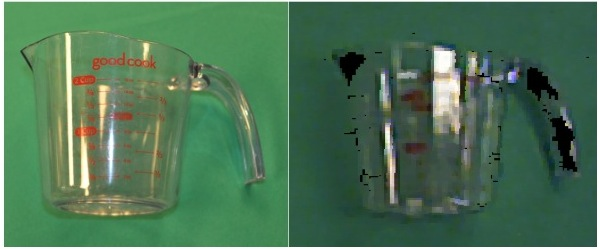
\includegraphics[width=8cm]{figures/cup.jpg} }}%
    
%       \qquad
  
     \subfloat{{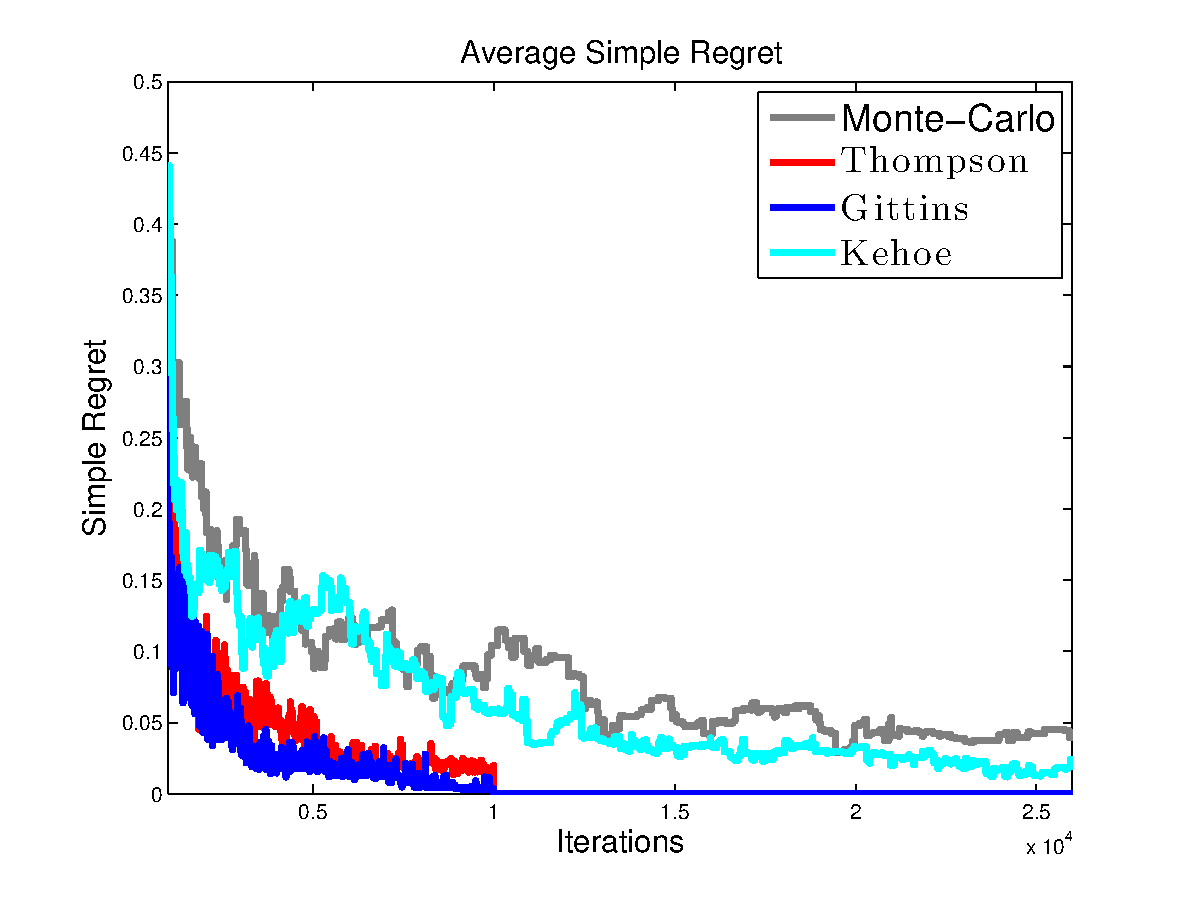
\includegraphics[width=8cm]{matlab_figures/teaser.eps} }}%
   
    \caption{\todo{New teaser photo, not sure if we should have some sort of real object or not}(Top Left) Image of a common household measuring cup. (Top Right) Image from a PR2 Primesense camera that reflects the uncertainty that can be induced in objects from transparency. (Bottom) Comparision of Multi-Armed Bandit Techniques (Bayes UCB, Thompson, Gittins) vs. Monte-Carlo sampling to determine the best grasp in a set of 1000 grasps. As you can see the bandit techniques converge in simple regret Eq. \ref{eq:simple_regret} a magnitude faster than the traditional approach of Monte-Carlo sampling to determine the highest quality grasp.  }%
    \label{fig:rot_shapes}%
\end{figure}

Analytic grasp quality metrics have been developed to determine the stability of a grasp when all the parameters of the object and robot manipulator are exactly known.
A common measure of stabliity in the literature is force closure, the abliity to resist external forces and torques in arbitrary directions~\cite{}.
Grasps in force closure can be further ranked by the relative magnitude of forces and torques that must be exterted by the gripper to resist external perturbations~\cite{ferrari1992}.
Recent works have explored computing the probability of a grasp achieving the force closure condition given uncertainty in parameters such as pose~\cite{christopoulos2007handling, weisz2012pose, kim2012physically} and object shape~\cite{kehoe2012estimating, mahler2015gp}.
Most methods for evaluating grasp quality in the presence of uncertainty use exhaustive Monte-Carlo sampling over the possible values of uncertain quantities~\cite{christopoulos2007handling, kim2012physically, weisz2012pose, kehoe2012estimating, kehoe2012towards} which can be very time consuming..
However, in many cases we may be able to rule out grasps with a low probability in only a few samples and allocate more sampling effort to grasps that are likely to be high quality.

The multi-armed bandit (MAB) model for sequential decision making problems~\cite{barto1998reinforcement, lai1985asymptotically, robbins1952some} provides a formal way to reason about allocating sampling effort to grasps such that the grasp(s) with highest quality can be determined in as few samples as possible.
In a standard MAB there are a set of possible options (or `arms' in the literature~\cite{barto1998reinforcement}) that each return a numeric reward from a stationary distribution.
The goal in a MAB problem is to sequentially select ones of the possible options such that a measure of expected reward is maximized.
Solutions to the MAB model are particularly useful in applications where it is too expensive to fully evaluate a set of options; for example, in optimal design of clinical trials~\cite{simon1989optimal}, market pricing~\cite{rothschild1974two}, and choosing strategies for games~\cite{st2012online}.
The budgeted multi-armed bandit model \cite{madani2004budgeted} is a specialization of the MAB model where an agent has a fixed number of decisions to make before choosing the best option.
The objective is to maximize the expected reward of the decision made at the stopping time, or equivalently to minimize ``simple regret", which is the difference between the true expected reward of an optimal arm and the true expected reward of the arm pulled at the stopping time.

Our main contribution is formulating the problem of ranking a set of candidate grasps according to a quality metric in the presence of uncertainty as a budgeted multi-armed bandit problem. %\todo{Jeff: probably needs to be more specific here, unless we formally describe how to do it in an arbitrary model}.
We study this formulation using probability of force closure~\cite{christopoulos2007handling, weisz2012pose, kehoe2012toward} as a quality metric under uncertainty in pose, shape, robot motion, and friction coefficient. 
We model shape uncertainty using Gaussian process implicit surfaces (GPISs), a Bayesian representation of shape uncertainty that has been used in various robotic applications~\cite{dragiev2011, hollinger2013}. 
Uncertainty in pose is represented as a normal distributions around the orientation and translation of the object.
Uncertainity in motion is represented as a normal distribution around the end point of a planned gripper trajectory and uncertainty in friction coefficient is a normal distribution around an expected friction coefficient.
\todo{Jeff: I personally think the above 3 statements may be too much detail for an intro}
However, our approach of treating grasp selection as a BMAB only requires the ability to sample from a given representation of uncertainty and is not restricted to aforementioned representations.
We compare the performance of several popular algorithms for solving the BMAB problem: Bayes UCB, Thompson sampling, and Gittins indices.
Our experiments demonstrate that solutions to the MAB problem can find the grasp with highest probabilty of force closure from a set of 1000 grasps 5x faster than the baseline Monte-Carlo approach and ...
\todo{Going to get a table with results. Make comparison to Ben's method}

\section{Related Work}

Past work on grasping under uncertainty has considered shape uncertainty \cite{goldberg1990bayesian, stulp2011learning}, uncertainty in contact locations with an object \cite{zheng2005}, and uncertainty in object pose \cite{christopoulos2007handling, weisz2012pose, kim2012physically}.
The effect of uncertainty in object geometry on grasp selection has been studied for spline representations of objects~\cite{christopoulos2007handling}, extruded polygonal mesh models~\cite{kehoe2012estimating, kehoe2012toward}, and point clouds~\cite{hsiao2011bayesian}.
A common method for evaluating a probabilistic grasp quality measure is to use Monte-Carlo sampling~\cite{christopoulos2007handling, kehoe2012estimating, kehoe2012toward}, which involves exhaustively sampling from distributions on random quantities and averaging the quality over these samples to approximate an expected value~\cite{caflisch1998monte}.
Exhaustive sampling can be computationally expensive, which motivated the use of Cloud Computing to distribute sampling effort~\cite{kehoe2012toward}.

To further address the computational complexity, Kehoe et al.~\cite{kehoe2012estimating} demonstrated a procedure for finding a minimum bound on expected grasp quality given shape uncertainty, which reduced the number of samples needed in Monte-Carlo sampling to choose the highest quality grasps. However, the proposed adaptive sampling approach pruned grasps using only the sample mean and did not utilize any estimates of how accurate the current sample mean is, which in practice could lead to good grasps being thrown away.
Laaksonen et al.~\cite{laaksonen2012probabilistic} used Markov Chain Monte-Carlo (MCMC) sampling to estimate grasp quality and object pose  under shape and pose uncertainty when the robot is able to obtain new information via tactile sensor.
MCMC provides a Bayesian framework for inference with a hidden state, but it can be slow to converge to the correct distribution due to burn in and mixing conditions~\cite{andrieu2003introduction}.

We chose to study our MAB sampling method on distributions for friction coefficient, pose, motion and shape. For shape uncertainty we decided to use a Gaussian process implicit surface representation. Our decision to use this uncertainty model is based on GPIS's ability to combine different modes of noise observations such as tactile, laser and visual~\cite{rasmussen2006, williams2007, dragiev2011} and its recent use in modeling uncertainty for a number of robotic applications.
Hollinger et al. used GPIS as a model of uncertainty to perform active sensing on the hulls in underwater boats \cite{hollinger2013}.
Dragiev et al. showed how GPIS can enable a grasp controller on the continuous signed distance function \cite{dragiev2011}.
Mahler et al. used the GPIS representation to find locally optimal anti-podal grasps by framing grasp planning as an optimization problem \cite{mahler2015gp}.  However, this relied on an approximation to grasp quality without guarantees on accuracy. We propose an adaptive sampling approach known as the Multi-Armed Bandit Model. This paper is a substantially revised and expanded version on \cite{laskey} and \cite{mahler2015gp}.




\section{Preliminaries and Problem Definition}
We consider selecting a grasp on object from a given set of candidate grasps.
We formulate this problem for grasping a planar object from above using parallel-jaw grippers.
We assume that the object is rigid and remains stationary throughout the grasp.
In this work we consider uncertainty in shape, pose, robot motion, and friction coefficient and we assume that distributions on these quantiites are given.
In this section, we formally define our grasping model, formalize our sources of uncertainty, introduce our metric for grasp quality, and finally define our grasp planning objective.

%Before we present the problem definition, we introduce a way to evaluate the quality of a grasp and our grasping model, the line of action. We also introduce a graphical model to represent the distributions on friction coefficient, motion, pose and shape. 


\subsection{Candidate Grasp Model}
Our candidate grasp model is illustrated in Fig.~\ref{fig:grasp_model}.
Let $d$ denote the dimensionality of the shape representations we are using to select grasps and $m$ denote the number of jaws on the robotic gripper.
In this work we formulate the MAB problem for 2-dimensional shapes using parallel-jaw grippers, so $d=2$ and $m=2$.
In this work we also assume a finite width for each parallel jaw $w_j \in \mathbb{R}$.

Similar to~\cite{christopoulos2007handling}, we parameterize a grasp using a {\it line of action} for each gripper jaw, where each line of action is a 1D curve $\gamma(t): [0,1] \rightarrow \mathbb{R}^d$ with endpoints $\gamma(0) = \ba$ and $\gamma(1) = \bb$.
The line of action defines the trajectory that a jaw follows as the gripper closes around a shape.
A {\it grasp plan} is the set of lines of action for each of the jaws, $\Gamma = \{\gamma_1(\cdot),...,\gamma_m(\cdot)\})$ \cite{}.
For parallel-jaw grippers, $\Gamma = \{\gamma(t), \gamma(1 - t)\}$, since the two jaws approach the shape in opposite directions.
Furthermore, in this work we consider only straight lines of action.
The line of action model allows us to compute perturbations to the contact points and normals that occur due to shape uncertainty.
%We chose of the line of action model because perturbations to a surface resulting from shape uncertainty lead to changes in the location of contact with a surface, and the line of action allows us to compute these new locations.

Given a grasp plan and a deterministic shape, we define the {\it contact points} as the spatial locations at which the jaws come into contact with the object when following the given plan, $\bc_1, ..., \bc_m \in \mathbb{R}^d$.
We also refer to the unit outward pointing surface normals at the contact points as $\bn_1, ..., \bn_m \in \mathbb{R}^d$ and the object center of mass as $\bz \in \mathbb{R}^d$.
Together these form the set of grasp parameters $g = (\bc_1, ..., \bc_m, \bn_1, ... \bn_m, \bz)$ that enable us to evaluate the forces and torques that a given grasp can apply to an object.

%\begin{figure}[ht!]
%\centering
%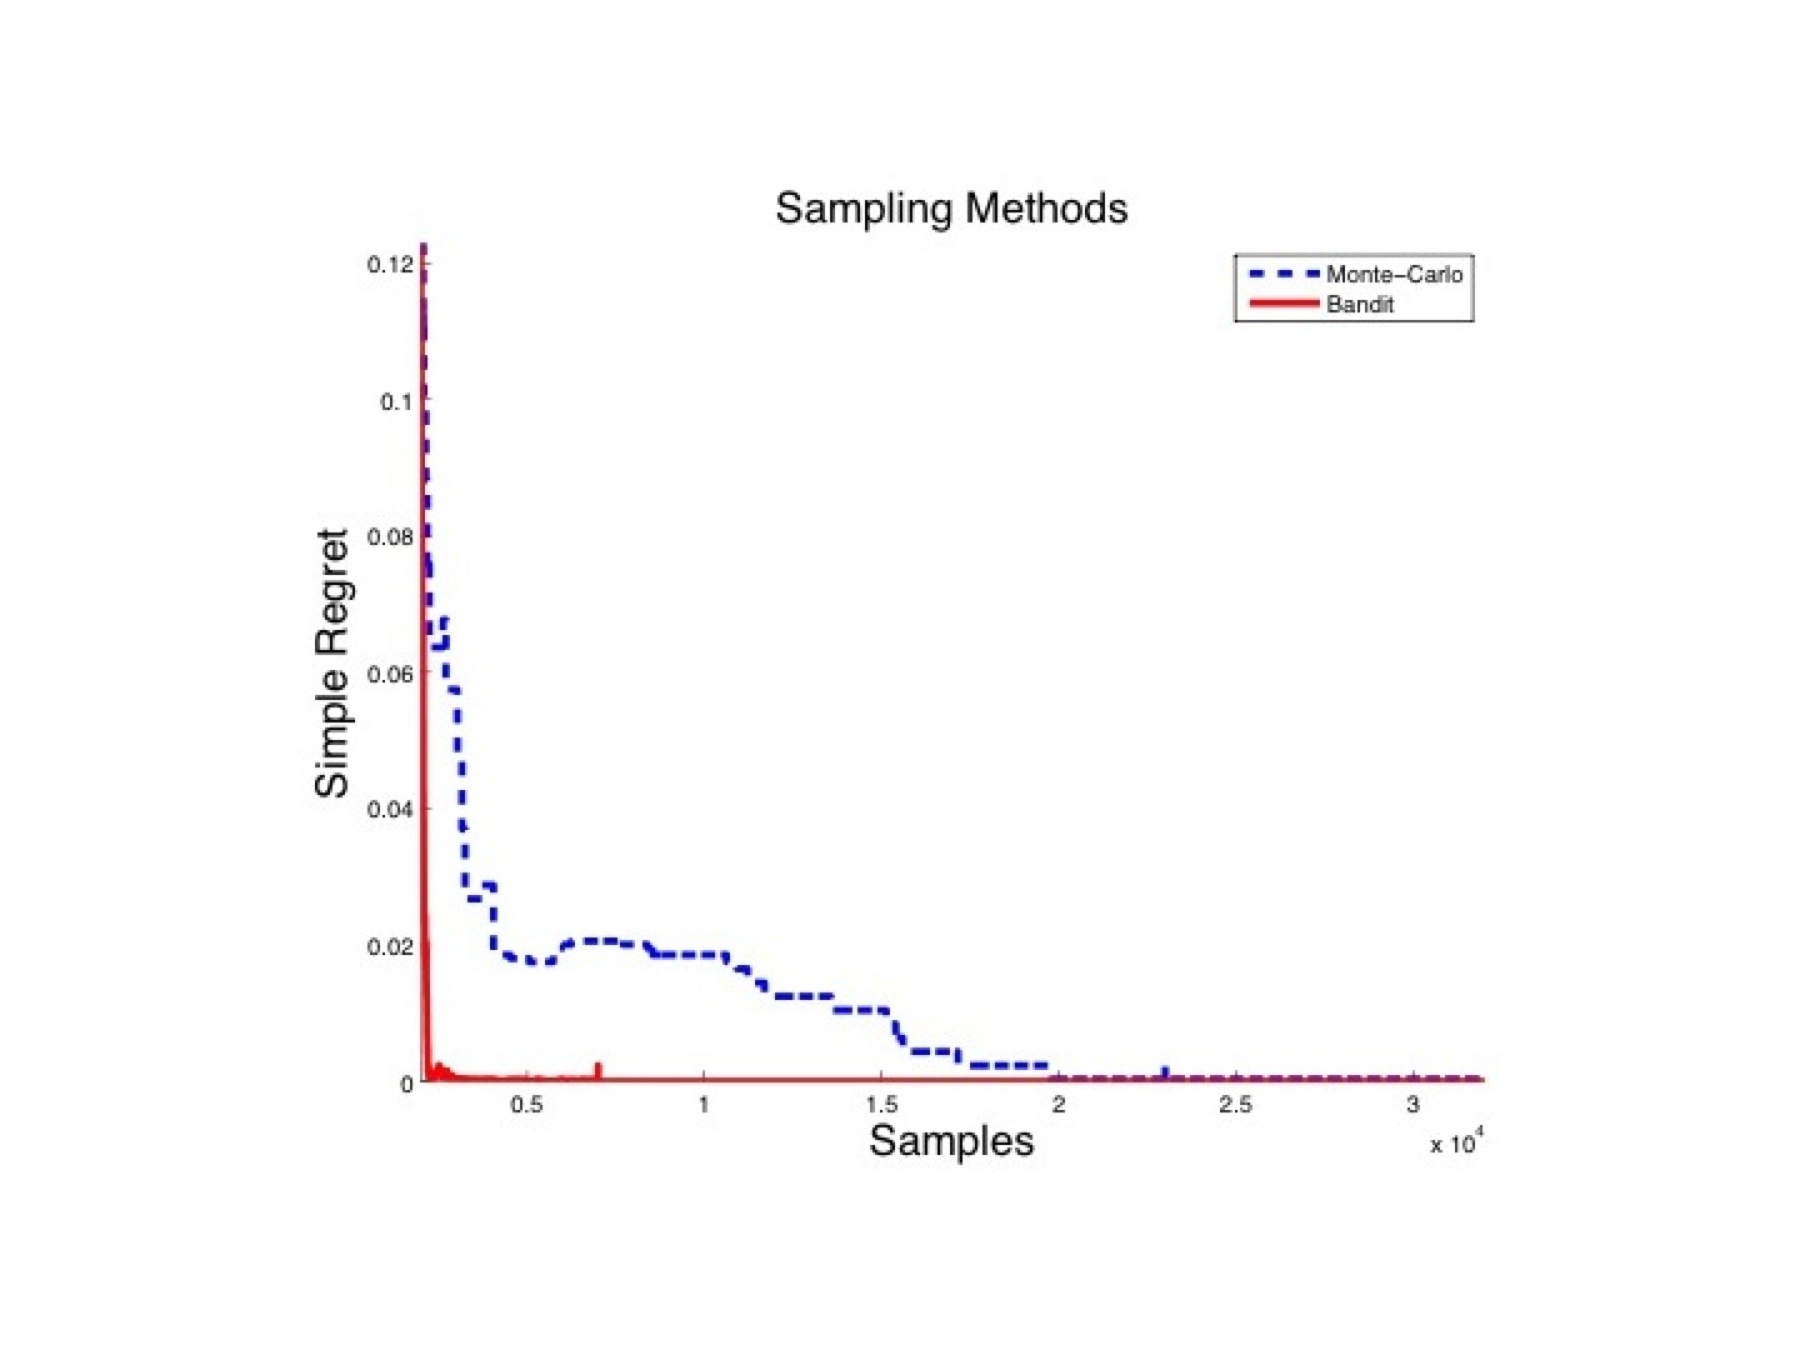
\includegraphics[width = 6cm, height = 4cm]{figures/Slide01.jpg}
%\caption{Illustration of a grasp plan $\Gamma$ composed of two lines of action, $\gamma_1(t)$ and $\gamma_2(t)$}
%\vspace*{-10pt}
%\label{fig:line_of_action}
%\end{figure}

\begin{figure}[t!]
\centering
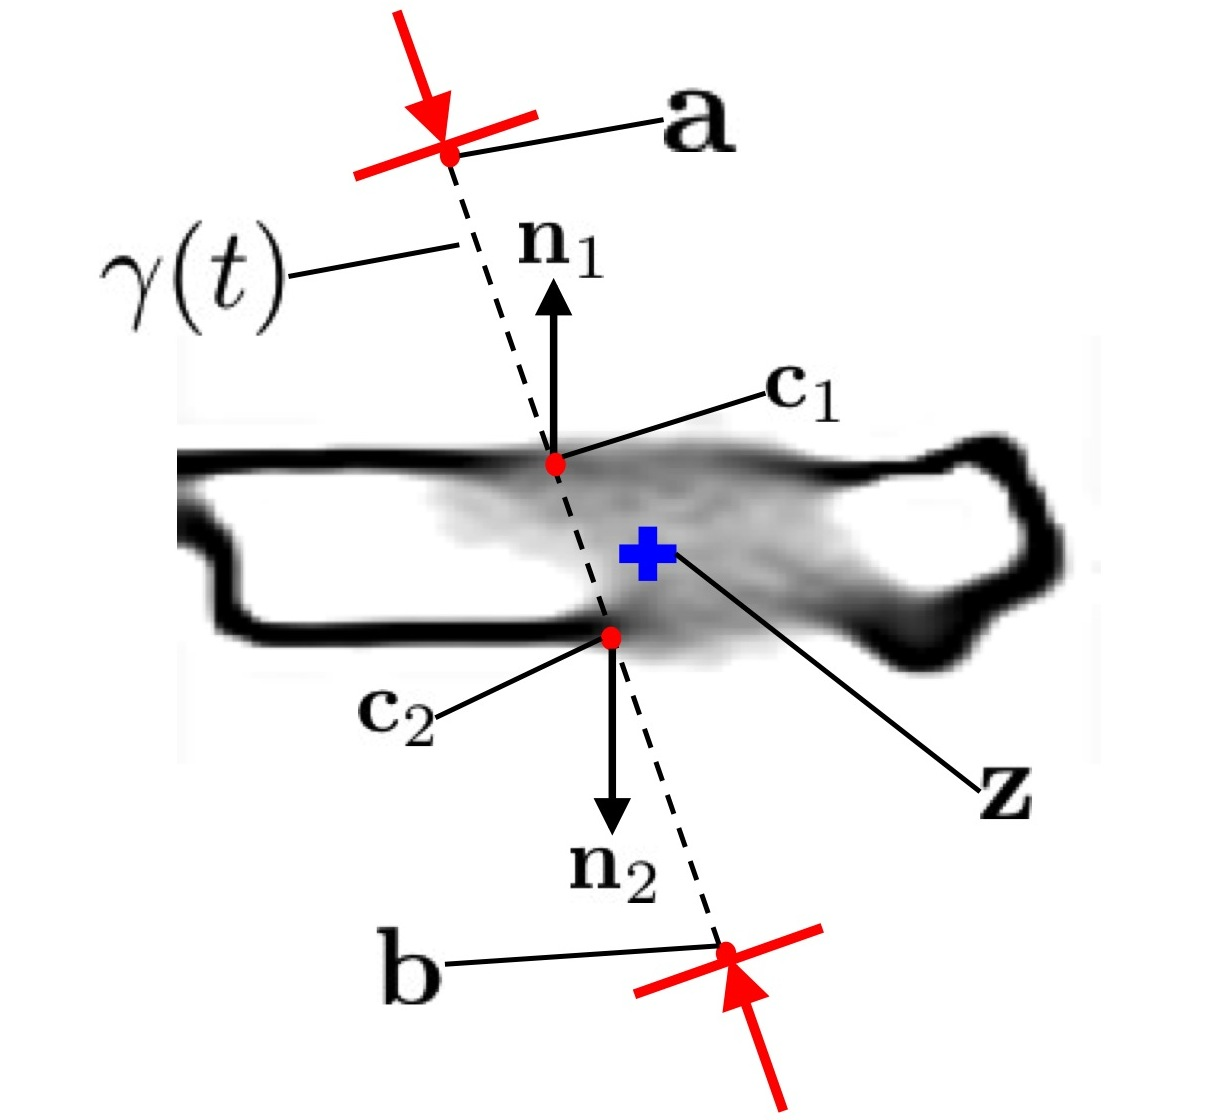
\includegraphics[width = 8cm, height = 6.5cm]{figures/grasp_model.jpg}
\caption{llustration of our grasping model for parallel jaw grippers on a GPIS model of a marker with shape uncertainty near the object center. Jaw placements are illustrated by a red direction arrow and line. The grasp plan consists of a line of action $\gamma(t)$ with endpoints $\ba$ and $\bb$. When following the grasp plan, the jaws contact the shape at locations $\bc_1$ and $\bc_2$ with outward pointing unit surface normals $\bn_1$ and $\bn_2$. Together with the center of mass of the object $\bz$, these values can be used to determine the forces and torques that a grasp can apply to an object. \todo{Jeff: Up to this point I don't believe the reader has seen a GPIS. We will replace the marker with a deterministic shape, but this figure gives a good idea of what we want to illustrate here.}}
\vspace*{-4ex}
\label{fig:grasp_model}
\end{figure}

\subsection{Sources of Uncertainty}
In this work we consider uncertainty in shape, pose, robot motion, and friction coefficient.
Fig. \ref{fig:graphical_model} illustrates a graphical model of the relationship between these sources of uncertainty.
In this section we describe each source of uncertainty and our model of the uncertainty.
We wish to emphasize that the models of uncertainty described in this work are not the only models that may be used with MAB algorithms and that the reader may choose parameters and distributions that best fit their needs. 

\subsubsection{Shape Uncertainty}

Uncertainty in object shape results from sensor noise and missing sensor data, which can occur due to transparency, specularity, and occlusions~\cite{mahler2015opt}.
Following ~\cite{laskey2015bandits, mahler2015opt} we represent the distribution over possible surfaces given sensing noise using a Gaussian process implicit surface (GPIS).
A GPIS represents a distribution over signed distance functions (SDFs), a surface representation commonly used in 3D reconstruction and SLAM \cite{}.
An SDF is a real-valued function $f: \mathbb{R}^d \rightarrow \mathbb{R}$ that is greater than 0 outside the object, 0 on the surface and less than 0 inside the object.
A GPIS is a gaussian distribution over SDF values at a fixed set of query points $\mX = \{\bx_1, ... \bx_n\}, \bx_i \in \mathbb{R}^d$, $f(\bx_i) \sim \mN(\mu_{f}(\bx_i),\Sigma_{f}(\bx_i))$, where $\mu_{f}(\cdot)$ and $\Sigma_{f}(\cdot)$ are the mean and covariance functions of the GPIS.
See Appendix A for detail on how to train a mean and covariance function for a GPIS.
In this work, we set $\mX$ to a uniform $M \times M$ grid of points with square cells.
For convenience, in later sections we will refer to the GPIS parameters as $\theta = \left( \mu_{f}(x), \Sigma_{f}(x) \right)$. 

\todo{Jeff: Describe alternative representation of shape uncertainty that we run experiments on. Likely this will be Ben's polygonal model}

\subsubsection{Pose Uncertainty}
In typical robotics applications the pose of objects in the envinroment is determined by registering the object frame-of-reference to the control frame-of-reference used for grasp execution.
Therefore pose uncertainty may come from either a) uncertainty about the registration of the robot's grasping frame-of-reference to its sensing frame-of-reference and b) uncertainty about the pose of known object models in the robot's sensor data.
In practice this uncertainty may be quantified based on the algorithms used to register these frames to one another.
The effects of pose uncertainty on robotic grasping has been studied by~\cite{weisz2012pose, kim2012physically}. % cite Ben's RSS workshop paper here

In 2-dimensional space, the pose of an object $T$ is a member of the Lie Algebra $SE(2)$.
This matrix is defined by a rotation angle $\phi$ and two translation coordinates $\bt = (t_x, t_y)$, summarized in parameter vector $\mathbf{\xi} = (\phi, \bt)^T \in \mathbb{R}^3$:

\vspace{-2ex}
\begin{align*}
	T &= \left[  \begin{array}{ccc}
		\cos(\phi) & -\sin(\phi) & t_x \\
		\sin(\phi) & \cos(\phi) & t_y \\
		0 & 0 & 1
		\end{array} \right] .
\end{align*}

One challenge with pose is that the pose matrix $T$ is used to apply pose perturbations to an object in practice, but uncertainty is mathematically more easily quantified in terms of the pose parameters $\xi$.
Folowing Barfoot and Furgale, we assume that we are given a mean pose matrix $\bar{T} \in SE(3)$ and zero-mean Gaussian uncertainty on the pose parameters $\mathbf{\xi} \sim \mN \left( \mathbf{0}, \Sigma_{\xi} \right)$, and we define the pose random variable $T$ as

\vspace{-2ex}
\begin{align*}
	T  &= \exp \left( \mathbf{\xi}^{\wedge} \right) \bar{T}
\end{align*}

\noindent where $\mathbf{\xi}^\wedge$ is the twist operator as defined in \cite{barfoot2014Pose}.

 
 \subsubsection{Motion Uncertainty}
In practice a robot may not be able to execute a desired grasp plan $\Gamma$ exactly due to slight errors in actuation or feedback measurements used for trajectory following~\cite{kehoe2012estimating}.
In this work, we model motion uncertainty as Gaussian uncertainty around the angle of approach and centroid of a straight line grasp plan $\Gamma$.
Formally, let $\hat{\by} = \frac{1}{2} (\ba + \bb)$ denote the center of a planned line of action $\gamma(t)$ and $\hat{\psi}$ denote the angle that the planned line $\bb - \ba$ makes with the x-axis of the 2D coordinate system on our shape representation.
Then the random center $\by \sim \mN(\hat{\by}, \Sigma_y)$ and the random angle $\psi \sim \mN(\hat{\psi}, \sigma_{\psi}^2)$.
For shorthand in the remainder of this paper we will refer to the random motion parameters as $\rho = \{\by, \psi \}$.
In practice $\Sigma_{y}^2$ and $\sigma_{\psi}^2$ might be set from repeatibility measurements for a robot \cite{mooring1986determination}.

 \subsubsection{Friction Uncertainty}
As shown in \cite{zheng2005}, uncertainty in friction coefficient can play a large role in grasp quality evaluation.
The expected friction coefficient $\hat{\mu}$ could be derived by means of object classification and a look up table~\cite{}.
However, friction coefficients may be uncertain due to factors such as material between a gripper and an object (e.g. dust, water, moisture), variations in the gripper material due to manufacturing tolerances, or misclassification of the object surface to be grasped.
We model uncertainty in friction coefficient as Gaussian noise, $\mu \sim \mN(\hat{\mu},\sigma_{\mu}^2)$. 
 
\subsection{Grasp Quality}
We measure the quality of grassp using the probability of force closure~\cite{weisz2012pose, kim2012physically, kehoe2012estimating, kehoe2012toward} given a grasp plan $\Gamma$, which we denote $P_F(\Gamma)$.
Force closure measures the ability to resist external wrenches, or force and torques vectors, assuming the grasp can apply infinite force.

Formally, force closure is a binary-valued quanity $F$ that is 1 if a grasp can resist wrenches in arbitrary directions and 0 otherwise.
Let $\mW \in \mathbb{R}^6$ denote the contact wrenches derived from contact locations $\bc_1, ... \bc_m$, normals $\bn_1, .., \bn_m$, friction coefficient $\mu$, and center of mass $\bz$ for a given grasp and shape.
If the origin lies within the convex hull of $\mW$, then the grasp is in force closure\cite{}.
In this work we rank grasps using the probability of force closure given uncertainty in shape, pose, robot motion, and friction coefficient~\cite{christopoulos2007handling, kehoe2012toward}:
%\vspace{-2ex}
\begin{align*}
	P_F(\Gamma) &= P(F = 1 | \Gamma, \theta, \xi, \rho, \mu).
\end{align*}
\todo{Jeff: revise above symbols for clarity} 
 
To estimate $P_F(\Gamma)$, we generate  samples from each of the above distributions in sequence using the relationships defined by the graphical model in Fig. \ref{fig:graphical_model}.
We first generate a sample of the object shape, pose, grasp plan, and friction coefficient using standard methods for sampling from a Gaussian distribution~\cite{}.
Then we use these quantities to determine the grasp parameters $g$. 
Finally, we compute the forces and torques that can be applied by $g$ to form the contact wrench set $\mW$ and evaluate the force closure condition.

To sample from $p(Q(\Gamma)>0)$, we need to sample from the distributions associated with a line of action $p(\textbf{n}_i,\textbf{c}_i|\gamma_i(t),\xi,\theta, \rho)$. Using Bayes rule  we can rewrite this as 
 
 \vspace{-2ex}
 \begin{align*}
 &p(\textbf{n}_i,\textbf{c}_i |\gamma_i(t),\theta,\xi,\rho)=\\
 &p(\textbf{n}_i|\textbf{c}_i,\theta)p(\textbf{c}_i|\gamma_i(t),\theta,\rho,\xi)
 \end{align*}

 
Appendix \ref{sec:Appendix}, describes how to draw shape sample from a GPIS model, which is used to compute $p(\textbf{c}_i|\gamma_i(t),\theta,\rho,\xi)$ along with the other sampled distribution on pose ($\xi$) and motion ($\rho$). Appendix \ref{sec:normals}, describes how to sample from $p(\textbf{n}_i|\textbf{c}_i,\theta)$ and presents a novel visualization technique for the distribution on surface normals.  Appendix \ref{sec:mass}, describes a way to calculate the expected center of mass assuming a uniform mass distribution. 
 \todo{Jeff: Not sure that the above two paragraphs are actually necessary}

%Let Q be the $L^1$ version of the metric depends on the contact points $\textbf{c}_1,...,\textbf{c}_m \in \mathcal{R}^2$, surface normals $\textbf{n}_1,...,\textbf{n}_m \in \mathcal{R}^2$, center of mass $\textbf{z}$ and friction coefficient $\mu$. The metric is evaluated by constructing a convex hull around the wrenches made up of those parameters and finding the radius of the largest unit ball centered at the origin in wrench space. If the convex hull  encloses the origin then the grasp is in ``force-closure,'' meaning the grasp can resist any external wrenches if enough force is used. A grasp can be parameterized by the following tuple $g = ( \textbf{c}_1,...,\textbf{c}_m,\textbf{n}_1,...,\textbf{n}_m,\mu, \textbf{z} )$\cite{pokorny2013classical}.
%
%In this work we use the probability of achieving force closure, or $P(Q>0)$, \cite{christopoulos2007handling}\cite{kehoe2012toward}, to rank grasps . $P(Q>0)$ may be computed by sampling from distributions on pose (rotation and translation of the object), shape and material properties (friction coefficient) and averaging the qualities that are computed.

\begin{figure}[ht!]
\centering
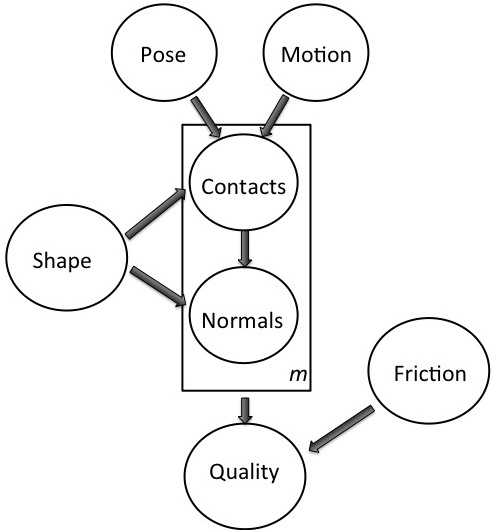
\includegraphics[width = 6cm, height = 6cm]{figures/Graphical_Model.jpg}
\caption{A graphical model that illustrates the relationship between the different types of uncertainty in an object. Center of Mass uncertainty is dependent on the pose and shape of the object, however friction coefficient is independent of all other types. \todo{Should we use words or symbols for the graphical model?}}
\vspace*{-10pt}
\label{fig:graphical_model}
\end{figure}

\subsection{Objective}

Given the sources of uncertainty and their relationships as described above, our goal is to find the grasp that maximizes the probability of force closure from a set of $P$ prespecified candidate grasps $\mG = \{\Gamma_1, ..., \Gamma_P\}$:

\vspace{-2ex}
\begin{align}
\Gamma^* &= \underset{\Gamma \in \mG}{\text{argmax }} P\left( F = 1 | \Gamma, \theta, \xi, \rho, \mu \right) \label{eq:problem_def}
\end{align}

One method to solve Equation ~\ref{eq:problem_def} is to exhaustively evaluate $P_F(\Gamma)$ for all grap plans in $\mG$ using Monte-Carlo integration and then sort the plans by this quality metric.
This method has been evaluated for shape uncertainty~\cite{christopoulos2007handling, kehoe2012estimating} and pose uncertainty~\cite{weisz2012pose} but is computationally expensive since it may require many samples for each of a large set of candidates to converge to the true value.
More recent works have considered adaptive sampling to discard grasp plans that are not likely to be optimal without fully evaluating their quality~\cite{kehoe2012toward} and searching for locally optimal grasp plans over a continuous set using Sequential Convex Programming~\cite{mahler2015opt}.
\todo{Jeff: differentiate from these}
In this work we show that this objective can be framed as a budgeted multi-armed bandit (BMAB) problem.

\section{Multi-Armed Bandits for Grasp Selection}
\label{sec:MAB}
%While a standard approach to solving the problem in Eq. \ref{eq:problem_def} would be to perform Monte-Carlo integration on each $\Gamma_i$ and compute the probability of force closure, we
We propose framing the problem in the multi-armed bandit (MAB) model and forming a policy for iteratively selecting which grasp to evaluate based on the probability of force closure estimate from the samples so far.
The goal of the MAB approach is to allocate more sampling effort to grasps that appear to have higher quality based on the evaluation performed so far.

\subsection{Standard MAB Model}
The multi-armed bandit model, originally described by Robbins \cite{robbins1985some}, is a statistical model of an agent attempting to make a sequence of correct decisions while concurrently gathering information about each possible decision.
Solutions to the multi-armed bandit model have been used in applications for which evaluating all possible options is expensive or impossible, such as the optimal design of clinical trials~\cite{simon1989optimal}, market pricing~\cite{rothschild1974two}, and choosing strategies for games~\cite{st2012online}. 

In a traditional MAB problem, a gambler has $K$ independent slot machines, or ``arms'' to play.
When an arm is played (or ``pulled'' in the literature), it returns an amount of money from a fixed reward distribution $P_k, k = 1, ..., K$ that is unknown to the gambler.
The goal of the gambler is to come up with a method for determining which arms to pull, how many times to pull each arm, and what order to pull them in such that the average cumulative rewards are maximized over many pulls.
If the gambler knew the machine with the highest expected reward, the gambler would only pull that arm.
However, since the reward distributions are unknown, a successful gambler needs to trade off exploiting the arms that currently yields the highest reward and exploring new arms to see if they give better rewards on average.
Developing a policy that successfully trades between exploration and exploitation to maximize average reward has been the focus of extensive research since the problem formulation \cite{bubeck2009pure}, \cite{robbins1985some}, \cite{bergemann2006bandit}.

Success in MAB problems is commonly measured in terms of {\it regret}, the difference between the expected optimal reward and the expected reward of the selected arm on a single pull.
Traditional bandit algorithms minimize cumulative regret, the sum of regret over the entire sequence of arm choices.
Lai and Robbins showed that an optimal solution to the bandit problem is bounded by a logarithmic function of the number of arm pulls~\cite{lai1985asymptotically}.
They presented an algorithm called (Upper Confidence Bound) UCB that obtains this bound asymptotically~\cite{lai1985asymptotically}.
The algorithm maintains a confidence bound on the distribution of reward based on prior observations and pulls the arm with the highest upper confidence bound.
Many variants of UCB have thus been proposed~\cite{}. \todo{Jeff: cite a lot of the literature here}
Since then a several other algorithms have been shown to achieve this bound, such as the Gittins index policy~\cite{} and Thompson sampling for certain reward distributions~\cite{}.

\subsection{Pure Exploration MAB Models}
Our grasp selection problem is similar in that we would like to find the grasp with the highest quality while conserving computational resources.
%Motivated by limited computational resources we allocate sampling resources to efficiently find the best arm.
However, in our problem one only cares about the suboptimality when the final grasp is selected for execution (called ``simple regret'' in the literature) rather than the cumulative regret as studied in the standard MAB problem.
This is an instance of the Pure Exploration multi-armed bandit problem\cite{bubeck2009pure}, in which an agent attempts to recommend the best arm at the end of an exploration phase but is not penalized for making exploratory arm pulls during this phase.
Hence, the exploration and exploitation stage are decoupled. 
The end of the exploration phase, or ``stopping time,'' may not be known to the agent ahead of time.
Therefore, unless otherwise noted, solutions to the Pure Exploration problem are anytime algorithms; they must return a valid solution whenever they are stopped.

Formally, given arms $\lbrace \Gamma_1, ..., \Gamma_K \rbrace$ with respective mean rewards $\mu_1, ..., \mu_K$, the goal in the Pure Exploration problem is to find the optimal arm $\mu^* = \underset{k\in\lbrace 1, ..., K \rbrace}{\mbox{max}} \mu_k$.
The expected simple regret, or suboptimality, at time $t$ is given by
%\vspace{-2ex}
\begin{align}\label{eq:simple_regret}
E[r_t] = \mu^* - \mu_t
\end{align}
\noindent where $\mu_t$ is the estimate of the best arm at time $t$ from the previous observations.

Several recent works have studied Pure Exploration algorithms that lead to upper bounds on the expected regret.
Audibert el al. demonstrated an algorithm called Successive Rejects that divides up the total budget into successively shorter phases and discards the worst arm left at the end of each phase.
This algorithm can return the best arm with near-optimal probability depending on the hardness of the problem and the number of allocated time steps \cite{audibert2010best}, but requires knowledge of the stopping time.
In addition, UCB-like methods have been proposed that measure a confidence gap and then pull the arm with the highest confidence interval \cite{gabillon2012best}.
For example, Bubeck et al. showed that the simple regret at any time for the UCB algorithm is bounded by a polynomial function of the number of timesteps~\cite{bubeck2009pure}.
Several works have showed the relationship between number of timesteps and simple regret for Probably Approximately Correct (PAC) bandit algorithms~\cite{even2006action, mannor2004sample}.
More recently, Bachman and Precup showed that algorithms based on Bayesian posterior sampling outperformed UCB and PAC algorithms in terms of minimizing simple regret~\cite{bachman2013greedy}.
%Even-dar et al. showed that for Probably Approximately Correct (PAC) algorithms, the number of pulls needed to 


%Best arm identification has a wide variety of literature that largely falls into two camps: one where the algorithm terminates once a fixed confidence interval around the best arm is met and the Budgeted Multi-Armed Bandit (BMAB) model, in which the algorithm must make a decision at the end of a fixed ``budget'' number of arm pulls.

%\subsection{Fixed Confidence}
%In the fixed confidence setting the forecaster seeks to minimize the simple regret until a fixed confidence threshold is met at which point it terminates. Originally the problem was solved with `racing' algorithms, which used Hoeffding inequalities or the empirical Bernstein inequality to prune arms that were likely to be suboptimal and used uniform allocation to explore the remaining set \cite{maron1993hoeffding} \cite{mnih2008empirical}. These methods were later extended to return the top $m$ arms instead of only the best arm\cite{gabillon2012best}. 
%
%The speed of termination is affected by the hardness of the problem, which relates to the how close the other arms expected reward is to the expected reward top arm in the set \cite{audibert2010best}. In the grasping context this means that achieving a fixed confidence for two similar grasps would require exhaustive sampling from each distribution. 
%
%\subsection{Fixed Budget}
%
%In the Budgeted Multi-Armed Bandit (BMAB) setting the algorithm is given a stopping time and needs to return the current best arm at that stopping time this can be thought of as an anytime algorithm.
%Audibert el al. demonstrated an algorithm called Successive Rejects that divides up the total budget into successively shorter phases and discards the worst arm left at the end of each phase.
%This algorithm can return the best arm with near-optimal probability depending on the hardness of the problem \cite{audibert2010best}.
%In addition, UCB-like methods have been proposed that measure a confidence gap and then pull the arm with the highest confidence interval \cite{gabillon2012best}. For example in \cite{bubeck2009pure}, they showed a link between simple regret and cumulative regret that allowed for the analysis of the existing bandit algorithms like UCB1.

\subsection{Grasp Planning as Pure Exploration}
In this work, we frame the grasp selection problem of \secref{objective} as a Pure Exploration multi-armed bandit problem.
Each arm corresponds to a different grasp plan and pulling an arm corresponds to sampling from the graphical model in Fig. \ref{fig:graphical_model} and evaluating the force closure condition.
Since force closure is a binary value, we can think of each grasp plan $\Gamma_i$ as having a Bernoulli reward distribution with probability of success $P_F(\Gamma_i)$.
Thus, the expected value of the force closure condition for grasp $\Gamma_i$ is $\mu_i = E[F | \Gamma_i, \theta, \xi, \rho, \mu] = P_F(\Gamma_i)$.
Then minimizing the expected simple regret is equivalent to maximizing $P_F$ over the set of candidate grasp plans:

\vspace{-2ex}
\begin{align*}
	\underset{\Gamma_i \in \mG}{\text{argmin }}\mu^{*} - \mu_{i} &= \underset{\Gamma_i \in \mG}{\text{argmax }}\mu_{i} \\
	&=  \underset{\Gamma_i \in \mG}{\text{argmax }} P_F(\Gamma_i) \\
	&= \Gamma^{*}
\end{align*}

In Section \ref{sec:bandit_algorithm}, we will discuss some of the most popular algorithms for solving the multi-armed bandit problem in detail. 

\section{Bayesian Algorithms for MAB}\label{sec:bandit_algorithm}

\todo{Jeff: I find this transition a bit awkward but I'm not sure how to reorg right now. I almost feel like Bayesian methods should come sooner}.
Most of the algorithms discussed in Section~\ref{sec:MAB} are frequentist, meaning the algorithms treat unknown parameters as fixed and use confidence intervals to score the arms. 
In this work, we are particularly interested in Bayesian algorithms that use previous samples to form a belief distribution on the likelihood of achieving force closure \cite{weber1992gittins,agrawal2011analysis}, as these methods have been shown empirically to outperform frequentist algorithms (e.g., UCB) on real datasets such as ad placement~\cite{chapelle2011empirical, bachman2013greedy}.
%However, recently Bayesian approachs have gained interest in the MAB community due to their empirical success on real world problems such as ad suggestions \cite{kaufmann2012bayesian} \cite{agrawal2011analysis}.
%In Bayesian algorithms, the agent maintains a belief distribution over the reward distribution on the arms.

Bayesian algorithms maintain a belief distribution on the grasp quality distributions for each of the candidate grasps to rank.
The belief distribution enables a trade off between exploration and exploitation by increasing confidence around the true reward distribution as more rewards are observed for an arms.
In the case of using force closure $F$ to measure quality, $P_F$ for each candidate grasp is a Bernoulli random variable and the Bayesian conjugate prior is a Beta distribution. 
Beta distributions are specified by shape parameters $\alpha$ and $\beta$, where ($\alpha >0$ and $\beta >0$).
Typically the uniform prior distribution on probability of force closure for each grasp $i$ at time $t = 0$, $\alpha_{i, 0} =1 $ and $\beta_{i, 0} = 1$, would be used used to initialize the algorithm~\cite{}. 
Theoretical results have shown that several algorithms for Beta-Bernoulli reward distributions are capable of achieving the lower bound described by Lai and Robbins~\cite{gittins1983dynamic, agrawal2011analysis, kaufmann2012bayesian}.
%Furthermore in an empirical study Bayesian methods have been shown to outperform the UCB family \cite{chapelle2011empirical}. 
%See \cite{} for a review of bayesian methods in multi-armed bandit problems. 

%In the context of grasping, the reward for achieving force close on a sample from the uncertain parameters is a Bernoulli random variable with probabilty of success $\theta$.
%%The distribution that describes whether an event is $\lbrace 0, 1 \rbrace$ is known as a Bernoulli distribution and can be described by the parameter $\theta$ or the probability an event occurs.
%In the Bayesian setting we treat $\theta$ as belonging to a distribution.
%A common choice for such a distribution is the Beta distribution, which is the conjugate prior of the Bernoulli distribution.
%One benefit of a conjugate prior is that the posterior update of the belief distribution is of the same form as the original prior, simplifying sampling and analysis.
%Beta distributions are specified by shape parameters $\alpha$ and $\beta$, where $\alpha >0$ and $\beta >0$.
%The mean of the Beta distribution is given by $\alpha/(\alpha+\beta)$.
%To update the prior Beta distribution one adds the count of observed successes of the event to $\alpha$ and the count of the observed failures to $\beta$
%Often the prior $\alpha =1 $ and $\beta =1$ is used before any rewards are observed, which leads to a uniform distribution on $\theta$. 

One benefit of the Beta prior on Bernoulli reward distributions is the elegant updates to the belief distribution after observing rewards from arm pulls.
Let $n_i$ denote the number of times grasp plan $\Gamma_i$ has been sampled.
Then after observing $S_i$ force closure conditions for grasp $\Gamma_i$, the posterior of the Beta can be computed as $\alpha_{i, n_i} = \alpha_{i, 0} + S_i, \beta_{i, n_i} = \beta_{i, 0} + n_i - S_i$, where $\alpha_{i,0}$ and $\beta_{i,0}$ are the prior shape parameters for $\Gamma_i$ before any samples are evaluated.
%Given a proposed grasp plan $\Gamma_i$ with current posterior belief $\alpha_i, \beta_i$, , we draw samples from the shape distribution $P(\theta)$, the distribution on pose $P(\xi)$, distribution on motion $P(\rho)$ and the distribution on friction coefficient $P(\mu)$.
%The distribution on force closure can then be estimated as Beta- Bernoulli Process with shape parameters $\alpha$ and $\beta$.
Given the current belief $\alpha_{i, n_i}, \beta_{i, n_i}$ on $P_F$ for a grasp plan $\Gamma_i$, the algorithm can predict the probability of force closure on the next iteration by taking the expected value:
\todo{Jeff: Revise notation. This was redone fairly quickly and may not be as clear as possible}
%Thus, we can write the expected probability of force closure as follows

\vspace{-2ex}
\begin{align}\label{eq:shape_sampling}
P_F(\Gamma_i) = \frac{\alpha_{i, n_i}}{\alpha_{i, n_i} + \beta_{i, n_i}}
\end{align}

Where $Q(\Gamma|\theta,\xi,\mu,z)$ is the grasp quality that is computed on a shape sample drawn from $p(\theta)$,$p(\xi)$,$p(\rho)$ and $p(\mu)$.
Whats interesting in the context of a Bayesian BMAB problem our graphical model in Fig. \ref{fig:graphical_model}, is now equivalent in terms of inference to \ref{fig:beta_model} and we only need to estimate $\alpha$ and $\beta$ to determine grasp quality.
\todo{Jeff: I see what you're trying to say here, but this is somewhat misleading. Alpha and beta constitue estimates of the probability of force closure but do not themselves determine grasp quality}
Regardless of the distributions in Fig. \ref{fig:graphical_model}, we are still able to maintain the theoretical guarantees given by the Bayesian MAB algorithms because the probability of force closure is a Beta-Bernoulli Process \cite{agrawal2011analysis} \cite{kaufmann2012bayesian} 
\cite{weber1992gittins}. 
\todo{Jeff: This is a strong statement but is pretty vague. What are these guarantees? I'd favor completely removing this paragraph.} 


\begin{figure}[ht!]
\centering
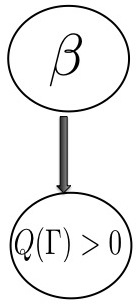
\includegraphics[width = 2cm, height = 4cm]{figures/Slide9.jpg}
\caption{A graphical model that illustrates the relationship between the Bernoulli distribution of the probability force closure and its conjugate prior Beta distribution that has two shape parameters $\alpha$ and $\beta$ }
\vspace*{-10pt}
\label{fig:beta_model}
\end{figure}


%In practice, when the distribution on the rewards of arms is not known, the empirical methods such as $\epsilon-$greedy have shown to have better performance in some situations \cite{kuleshov}.

%In our case we only care about the regret at the time our decision of the optimal grasp needs to be made, decoupling the exploration and exploitation stages.

We describe three popular Bayesian MAB algorithms below for the Beta belief distribution.

\todo{Jeff: Revise below sections for clarity}
\subsection{Bayes-UCB}
Bayes UCB, detailed in Algorithm 1, is a version of the UCB algorithm that uses a Bayesian posterior update to get a confidence bound instead of  the frequentist concentration inequality approach. To get an upper confidence bound from the posterior, the Bayes UCB algorithm uses the quantile of the Beta distribution up to a specified probability which depends on the timestep and horizon. At each time step the arm with the highest quantile is chosen and the Beta distribution is updated based on the observed reward.  For binary rewards (i.e. Bernoulli distributions) the expected number of pulls of suboptimal arms is bounded and experimentally this algorithm has been shown to outperform UCB for binary rewards \cite{kaufmann2012bayesian}.

\begin{algorithm}
 \KwResult{Current Best Arm, $\Gamma^*$ }
 For Beta(1,1) prior, Stopping Horizon $n$: \\
\For{ t=1,2,...,n}{ 
	\For{j = 1,...,K}{
	
		Compute: $q_j(t) = Q\big(1-\frac{1}{t},p_j^{t-1}\big)$
	
	}
Draw arm$ I_t = \mbox{argmax}_{j=1...K}q_j(t)$\\
 Observe reward $X_{I_t,t} \in \lbrace 0,1 \rbrace$\\
 Update posterior:\\
 Set $S_{I_t,t+1} = S_{I_t,t} + X_{I_t,t}$ \\
 Set $F_{I_t,t+1} = F_{I_t,t} + 1 - X_{I_t,t}$\\
 Set $\theta_j^t \sim \mbox{Beta}(S_{I_t,t+1},F_{I_t,t+1} )$\\
 }
 \caption{Bayes-UCB for Beta-Bernoulli Process}
\end{algorithm}


\subsection{Thompson Sampling}
Thompson Sampling is a Bayesian method for the multi-armed bandit problem. We will describe it now in detail for the Beta-Bernoulli process. All arms are initialized with a prior Beta distributions, which is normally Beta($\alpha=1$,$\beta =1$) to reflect a uniform prior on the $\theta$ of the Bernoulli distribution. Then for each arm draw $\theta_{j,t} \sim \mbox{Beta}(\alpha,\beta)$ and pull the arm with the highest $\theta_{j,t}$ drawn. The reward, $X_{i,t}$ is observed from that arm, $j$, and the corresponding Beta distribution is updated. This is repeated until a stopping time is reached. The full algorithm is shown in Algorithm 1.  

The randomness of Thompson sampling allows for it to quickly explore the more arms then Bayes-UCB, which makes conservative arm pulls based on confidence bounds. It is also less prone to local solutions because of its stochastic nature. Thus, for cases where exploration and exploitation are decoupled Thompson sampling can find a better arm faster. Thompson sampling has recently been shown to approach the Lai and Robbins bound \cite{agrawal2011analysis} and has  empirically been shown to outperform frequentist methods like UCB in certain settings \cite{chapelle2011empirical}. Variants of it are even used commercially in products like Microsoft's adPredictor, which is used by Bing, the search engine, \cite{graepel2010web}. 
\begin{algorithm}
 \KwResult{Current Best Arm, $\Gamma^*$ }
 For Beta(1,1) prior: \\
\For{ t=1,2,...}{ 
 Draw $\theta_{j,t} \sim$ Beta($S_{j,t}+1$,$F_{j,t}+1$) for $j = 1,...,k$\\
 Play $I_t=j$ for $j$ with maximum $p_{j,t}$\\
 Observe reward $X_{I_t,t} \in \lbrace 0,1 \rbrace$\\
 Update posterior:\\
 Set $S_{I_t,t+1} = S_{I_t,t} + X_{I_t,t}$ \\
 Set $F_{I_t,t+1} = F_{I_t,t} + 1 - X_{I_t,t}$\\
	
 }
 \caption{Thompson Sampling for Beta-Bernoulli Process}
\end{algorithm}



\subsection{The Gittins Index Method} 
\todo{Let me know how clear this is, Gittins can be hard to describe in general}
\todo{Jeff: Needs some work. We will have to think about how to get this across intuitively.}
One possible solution to solve the MAB problem is to treat it as an Markov Decision Process (MDP) and use Markov Decision theory. This solution makes a lot of sense when the distribution is known because the all elements in the standard MDP tuple, $\lbrace S,A,T,R,\gamma \rbrace$, would be known and it is optimal with respect $\gamma$ \cite{weber1992gittins}. 

However, the curse of dimensionality effects performance because if you have $K$ arms, a finite horizon of $T$ and a Beta-Bernoulli distribution on your arms then your state space is on the order of $T^{2*K}$. Hence the complexity of solving MAB using Markov Decision theory increases exponentially with the number of bandit processes. A key insight though was given by Gittins, who showed that instead of solving the $k$-dimensional MDP one can instead solve $k$ 1-dimensional optimization problems: for each arm $i$, $i= 1,...,k$, and for each state of $x^i = \lbrace \alpha_0 +S_t, \beta_0 +F_t \rbrace^i$, where $S_t$ and $F_t$ correspond to the number of success and failures at pull $t$. 


\vspace{-2ex}
\label{eq:git_indices}
\begin{align}
	v^i(x^i) = \underset{\tau>0}{\mbox{max}} \frac{\mathcal{E}[\sum_{t=0}^{\tau}\gamma^tr^i(X_t^i)|X_0^i = x_i]}{\mathcal{E}[\sum_{t=0}^{\tau}\gamma^t|X_0^i = x_i]}
\end{align}


The indices can be considered as a computation of the value in choosing an arm conditioned on the fact that you will give up an choose another arm at some point. Once you know the state of your $k$ arms, the algorithm is to select the one with the highest index.  For Best Arm Identification you want your discount factor $\gamma$ to approach 1, since you should never stop pulling the best arm. Generally the computation of the Gittins indices is too expensive, however in the Beta-Bernoulli case it is actually possible \cite{kaufmann2012bayesian}. We computed the Gittins indices offline using the restart method proposed by Katehakis et al. \cite{katehakis1987multi}.


\begin{algorithm}
 \KwResult{Current Best Arm, $\Gamma^*$ }
 For Beta(1,1) prior, Table of Indices $v$, Discount Factor $\gamma$: \\
\For{ t=1,2,...}{ 
 Pull arm $k = \underset{x_k \in X}{\mbox{argmax}} v(x_k)$\\
 Observe reward $R_{I_t,t} \in \lbrace 0,1 \rbrace$\\
 Update posterior:\\
 Set $S_{I_t,t+1} = S_{I_t,t} + R_{I_t,t}$ \\
 Set $F_{I_t,t+1} = F_{I_t,t} + 1 - R_{I_t,t}$\\
 Set $x_k = \lbrace 1 + S{I_t,t+1}, 1+F_{I_t,t+1} \rbrace$\\	
}
 \caption{The Gittins Index Method for Beta-Bernoulli Process}
\end{algorithm}

 .
\section{Experiments}
For the experiments we used the Brown Vision Lab 2D dataset, the same used in \cite{christopoulos2007handling}. We downsampled the image by a factor of 2 to create a 40 x 40 occupancy map, which holds 1 if the point cloud was observed and 0 if it was not observed, and a measurement noise map, which holds the variance 0-mean noise added to the SDF values. The parameters of the GPIS were selected using maximum likelihood on a held-out set of validation shapes. The noise of the motion, position and friction coefficient was set to the following variances $\sigma_{mu} = 0.4$, $\sigma_{rot} = 0.3$ rads,$\sigma_{trans} = 3$. Our visualization technique follows the approach of \cite{mahler2015gp} and consisted of drawing many shape samples from the distribution and blurring accordingly to a histogram equalization scheme. 

We did experiments for the case of two hard contacts in 2-D, however our methods are not limited to this implementation. We drew random lines of actions $\gamma_1(t)$ and $\gamma_2(t)$ by sampling around a circle with radius $\sqrt{2}n$ and sampling the circles origin, then projecting onto the largest inscribing circle in the workspace. 

\subsection{Multi-Armed Bandit Experiments}
\todo{add Bayes and Kehoe results}
We consider the problem of selecting the best grasp plan, $\Gamma^*$ out of a set $G$. For our experiments we look at selecting the best grasp out of a size of $|G| = 1000$. In Fig. \ref{fig:simple_regret}, we plotted the simple regret averaged over 100 randomly drawn shapes in our data set and compare the different methods (UCB, Thompson, Gittins and the naive random allocation). We initialize both the Monte-Carlo and bandit technique by sampling each grasp 1 time. We draw samples from our calculated distributions $p(g)$.  Interestingly, Gittins and Thompson converge much faster than random and UCB. In Fig. \ref{fig:pulls_per_grasp}, you can see that Gittins and Thompson allocate grasp samples to only the grasps of high quality, thus they are quickly able to ignore the low quality grasps. UCB takes a more conservative approach to sample allocation, which leads to poor performance in the best arm identification problem \cite{bubeck2009pure}.

\begin{figure*}[ht!]
\centering
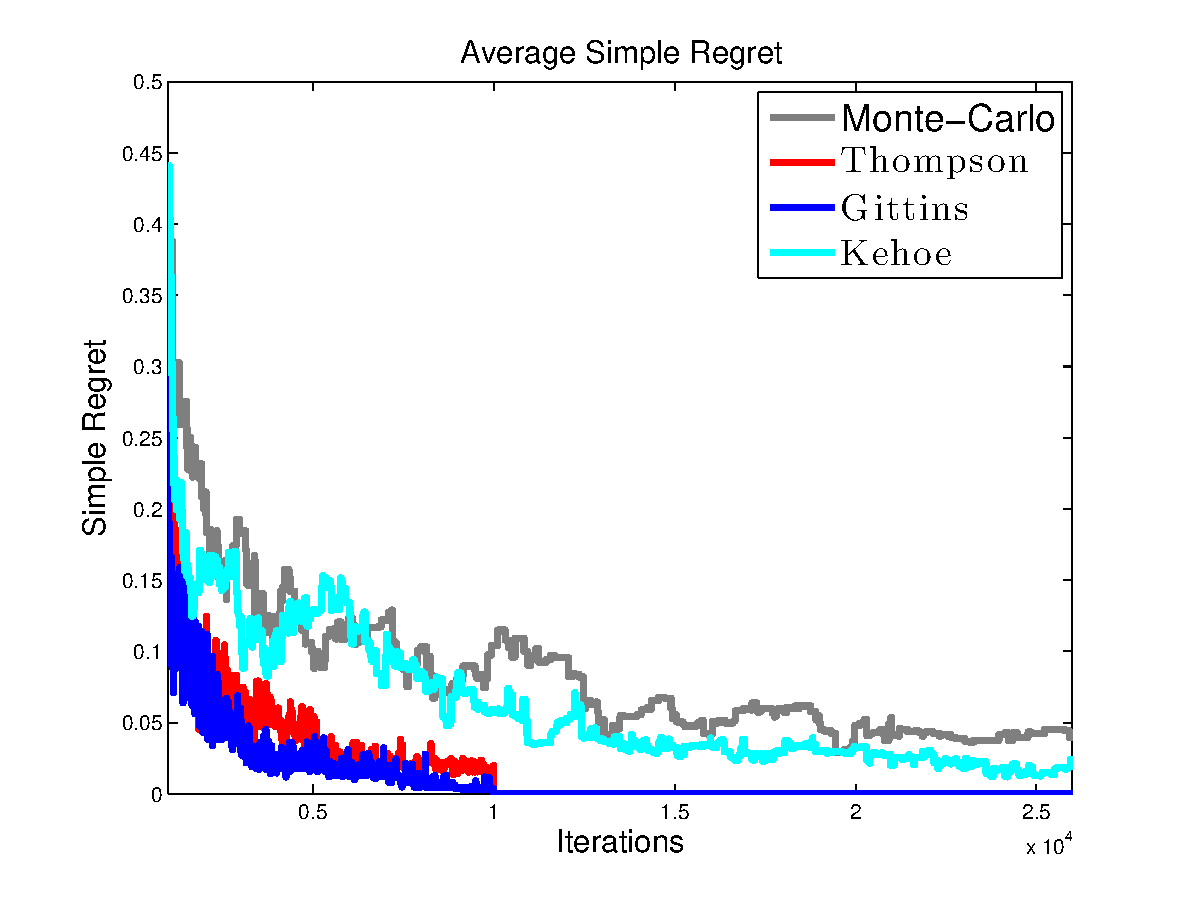
\includegraphics[width = 16.5cm, height = 9cm]{matlab_figures/simple_regret.eps}
\caption{ \footnotesize Comparison of Simple Regret convergence for the four sequential decision methods (Monte-Carlo, Bayes -UCB, Thompson, Gittins). Graph is averaged over 100 shapes from the Brown Sillohoute Dataset \cite{brown} with a set $|G|=1000$ for each shape. As you can see the BMAB methods converge almost a magnitude faster than random allocation. It is worth noting that Gittins outperform the other two algorithms, which is useful when choosing which one to implement }
\vspace*{-10pt}
\label{fig:simple_regret}
\end{figure*}


\begin{figure*}[ht!]
\centering
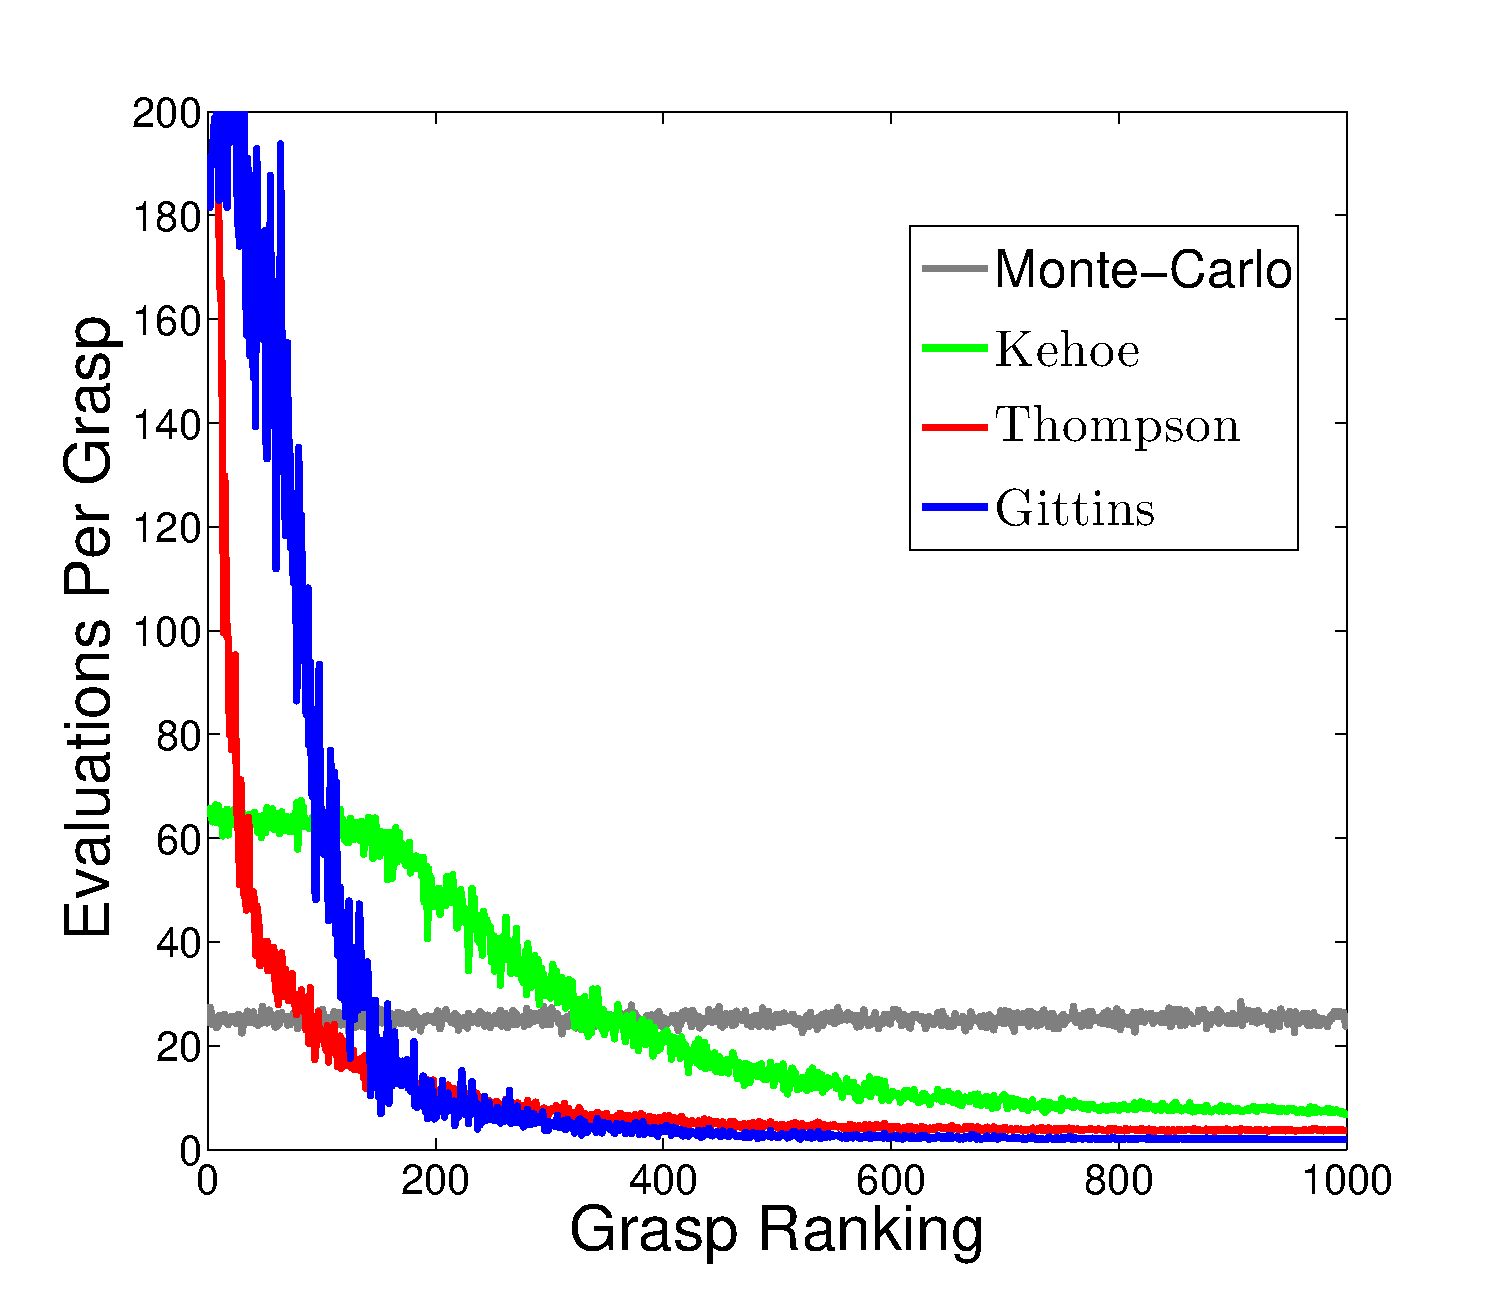
\includegraphics[width = 16.5cm, height = 9cm]{matlab_figures/pulls_per_grasp.eps}
\caption{ \footnotesize Comparison of sample per grasp for the four sequential decision methods (Random, Bayes - UCB, Thompson, Gittins). Graph is averaged over 100 shapes from the Brown Silhouette Dataset \cite{brown} with a set $|G|=1000$ for each shape. The best grasps are ranked 1 and worst are 1000. As you can see the MAB algorithm intelligently allocate samples towards high quality grasps based on past observations, where Monte-Carlo Integration takes a uniform approach to allocation. \cite{best_arm}}
\vspace*{-10pt}
\label{fig:pulls_per_grasp}
\end{figure*}
\begin{figure*}%
    \centering
    \subfloat{{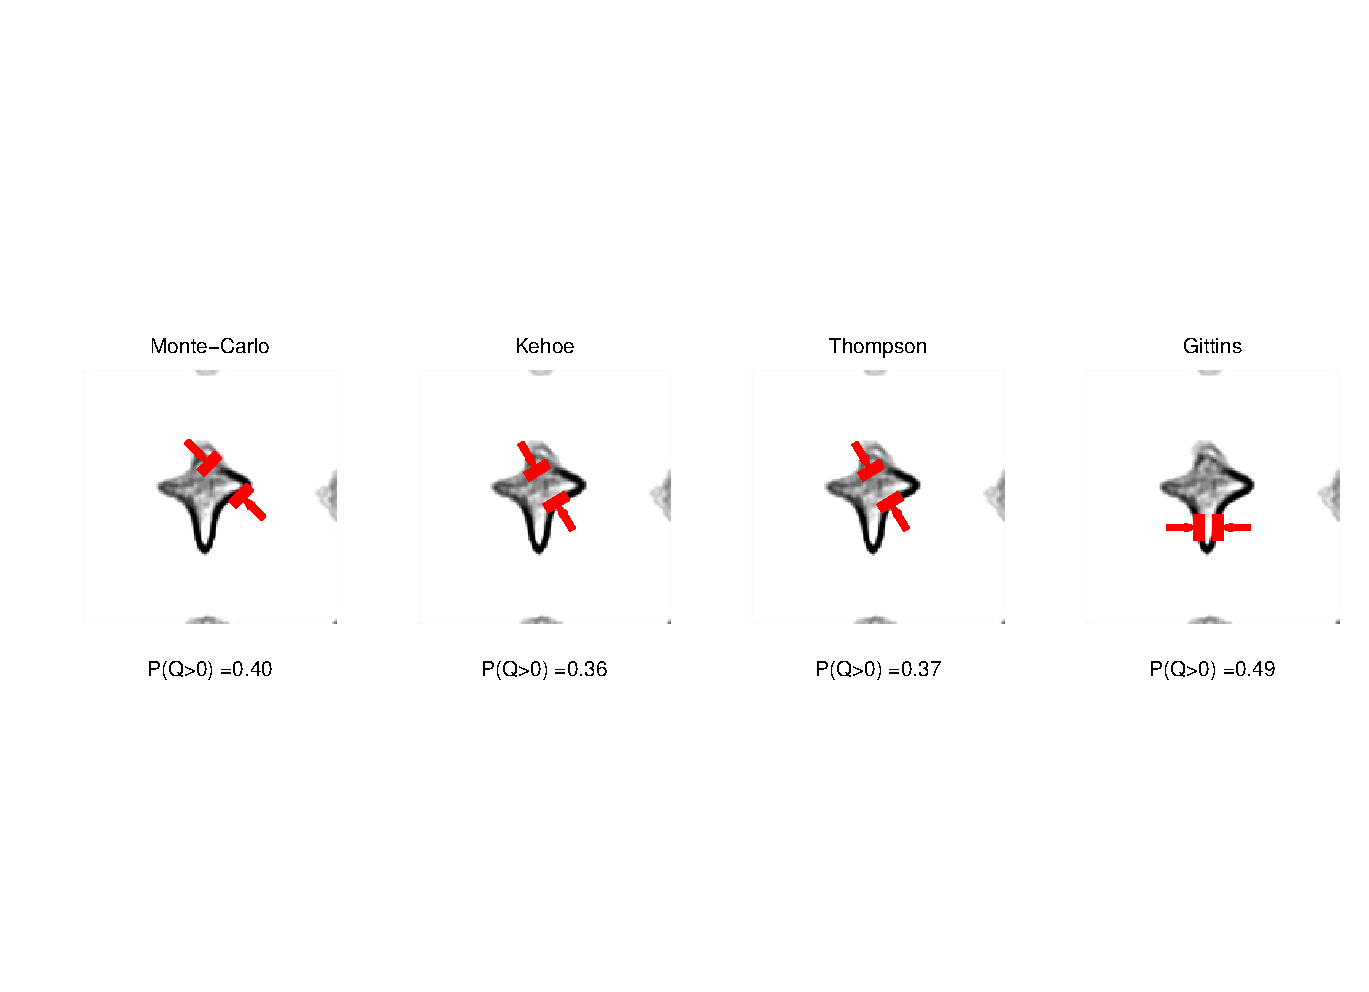
\includegraphics[width=16.5cm]{matlab_figures/shapes_1.eps} }}%
    \qquad
    \subfloat]{{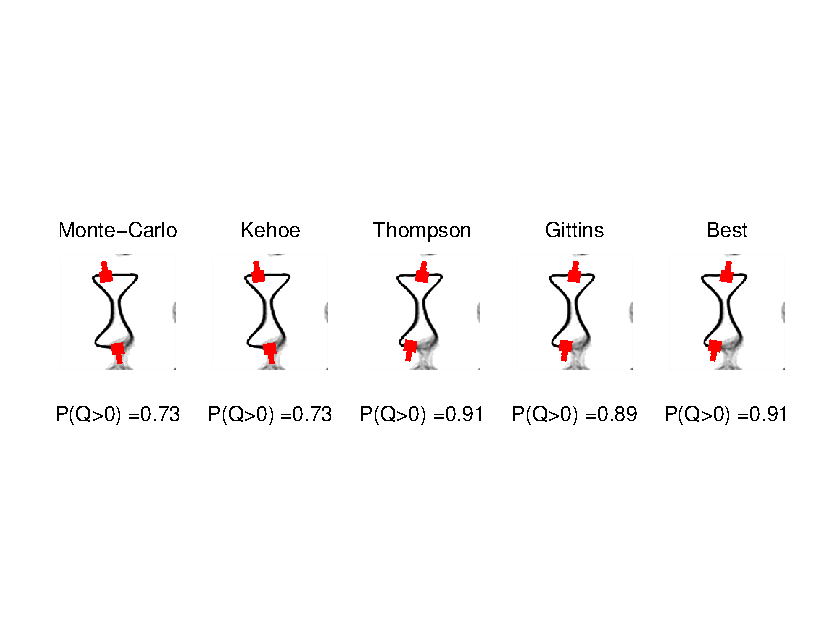
\includegraphics[width=16.5cm]{matlab_figures/shapes_2.eps} }}%
       \subfloat]{{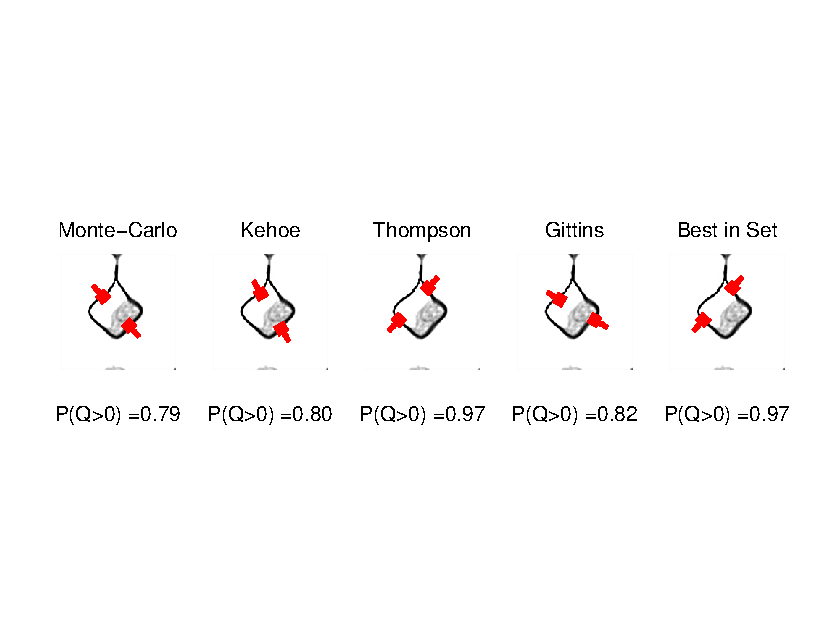
\includegraphics[width=16.5cm]{matlab_figures/shapes_3.eps} }}%
          \subfloat]{{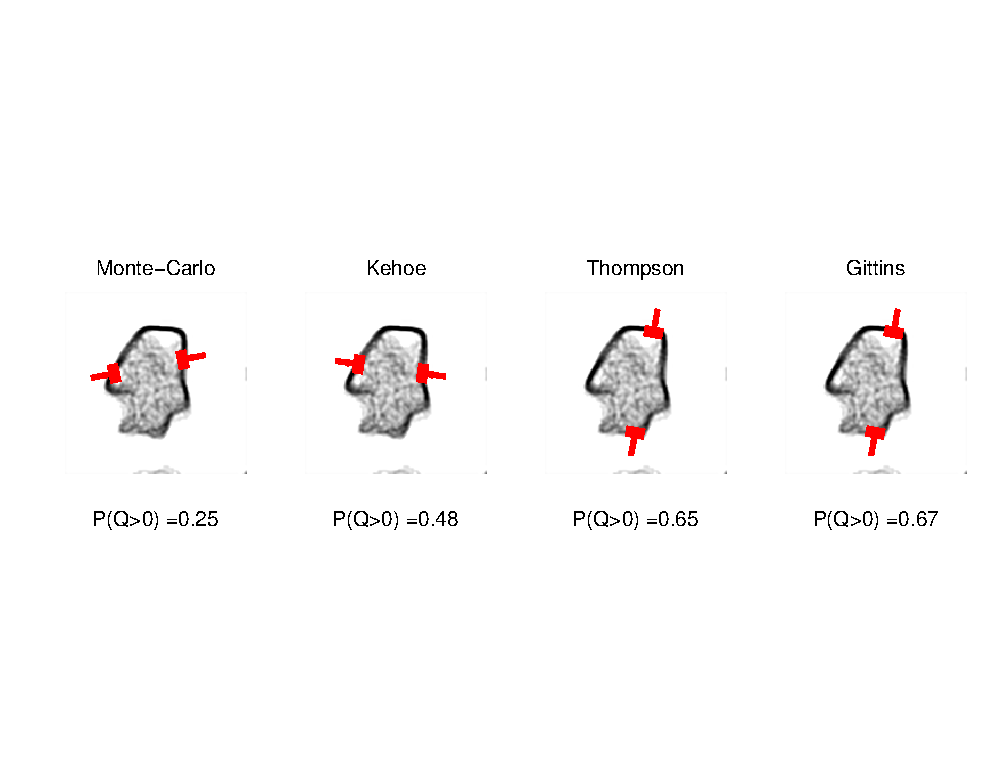
\includegraphics[width=16.5cm]{matlab_figures/shapes_4.eps} }}%
             \subfloat]{{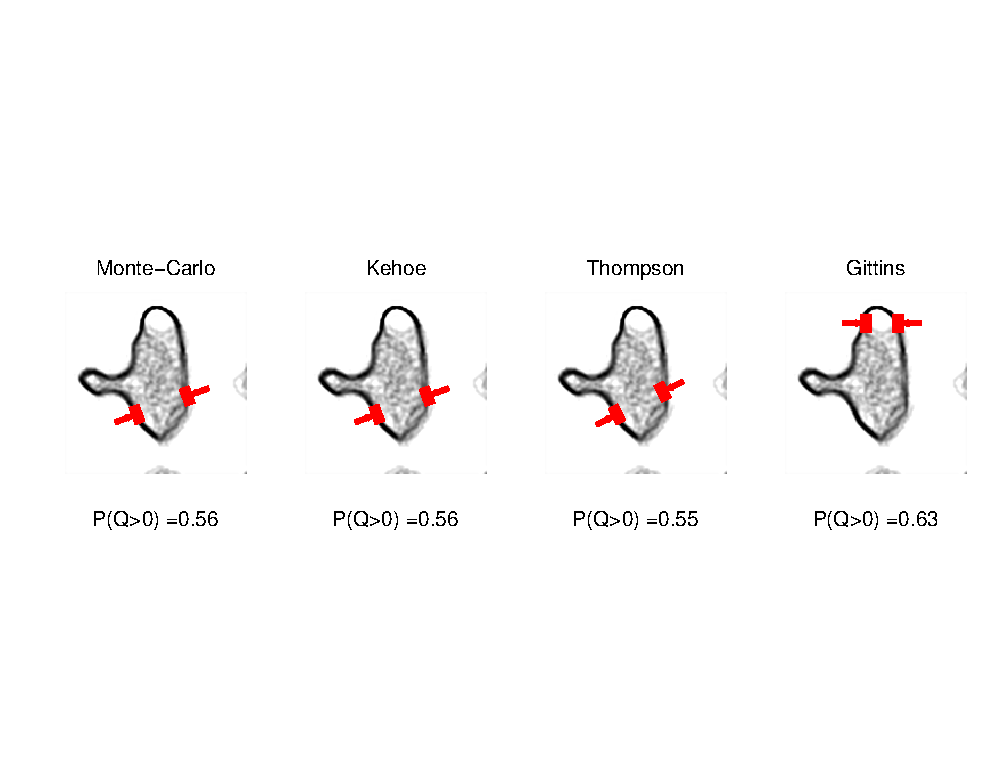
\includegraphics[width=16.5cm]{matlab_figures/shapes_5.eps} }}%
    
    \caption{Five shapes shown from the Brown Visual Lab Dataset with induced shape uncertainity and visualized according to the method described in \cite{mahler2015gp}. The four methods (Monte-Carlo, Kehoe's, Thompson and Gittins) were all run until a stopping time of 9000 evaluations with a uniformly initialized grasp set of $|G|=1000$. The grasps and the quality each one found is shown above. The Gittins Index Method in all cases shown found the best grasp among the methods.  }%
    \label{fig:rot_shapes}%
\end{figure*}

\subsection{Sensitivity Analysis }
We now will show how well the top two algorithms Thompson Sampling and the Gittens Index Method perform under a variation in noise from friction coefficient uncertainty, shape uncertainty, rotational pose and translation pose. The experiments are performed with the same setup as before but now we increase the variance parameters across a set range for each parameter to simulate low, medium and high levels of noise. All experiments were averaged across 10 shapes with a set size $|G| = 1000$. 

For friction coefficient we varied the variance across the following values $\sigma_{\mu} = \lbrace 0.05, 0.2, 0.4$. As illustrated in Fig. \ref{fig:fric_sens}, the performance of the bandit algorithm remains largely unchanged, with typical convergence to zero in simple regret less than 2000 evaluations.

For rotational uncertainity in pose, we varied $\sigma_{rot}$ over the set of $\lbrace 0.03, 0.12,0.24\rbrace$ radians. As you can see in Fig. \ref{fig:rot_sens}, the performance of the bandit algorithms is effected by the change in rotation, increase in variance to $0.24$ radians or $13^{\deg}$  causes the convergence in simple regret to not be reached until 5500 samples or an average of 5.5 samples per grasp. This can be explained because such a large variance causes a a drop in quality across all grasps and makes it harder to separate the outliers \cite{gabillon2012bes}. The quality of the best grasp along with the grasp for each round is shown in \ref{fig:rot_shapes}. 


For translational uncertainty in pose, we varied $\sigma_{trans}$ in the range of $\lbrace 3,12, 24 \rbrace$ units (on a 40 x 40 unit workspace). As you can see in Fig. \ref{fig:rot_sens}, the performance of the bandit algorithms is effected by the change in rotation, increase noise of $\sigma_{trans} = 24$ causes the convergence to not be reached until around 5000 samples for the Gittens Method and  8200 evaluations for Thompson Sampling.







\begin{figure}[ht!]
\centering
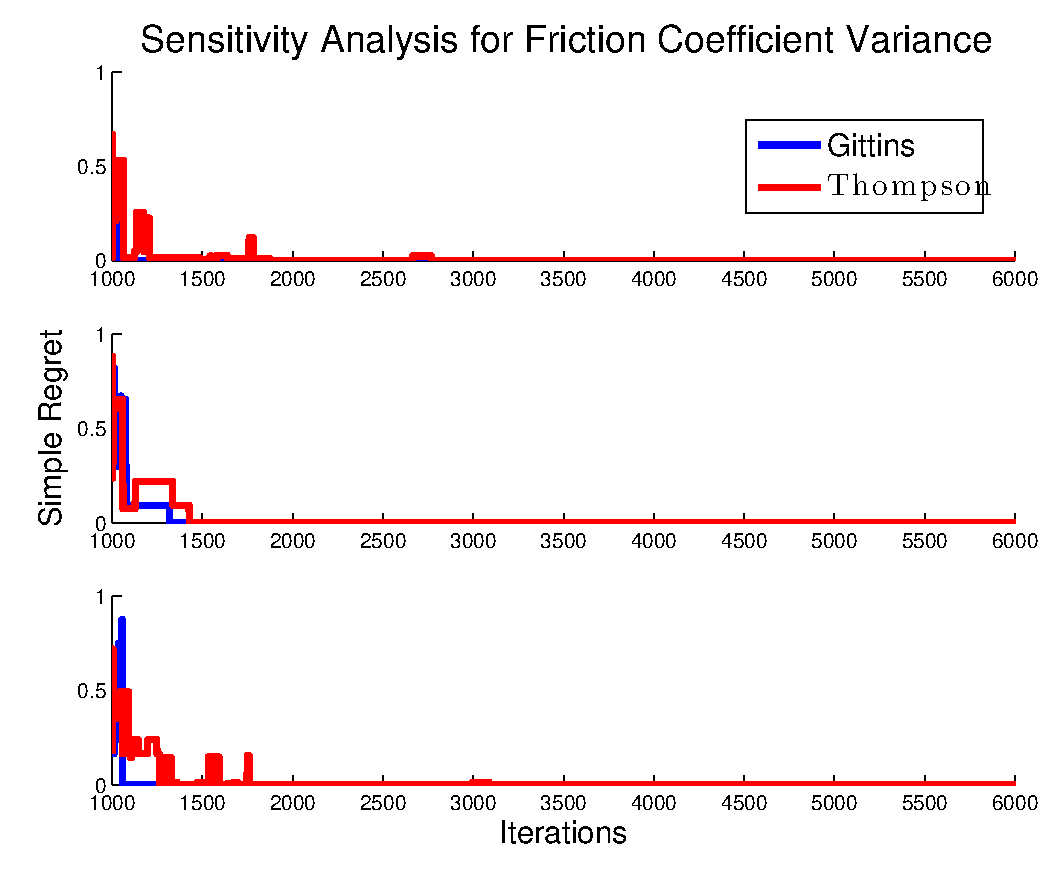
\includegraphics[width = 8cm, height = 10cm]{matlab_figures/sensitivity_fric.eps}
\caption{ \footnotesize Sensitivity Analysis for Thompson Sampling and the Gittens Index Method under friction coefficient uncertainty $\sigma_{fric} = \lbrace 0.05,0.2, 0.4 \rbrace$  from top to bottom on a 40 x 40 unit workspace averaged over 10 shapes from the Brown Vision Lab Data set. The increase in noise has little effect on the convergence of the two algorithms in simple regret.}
\vspace*{-10pt}
\label{fig:fric_sens}
\end{figure}

\begin{figure}[ht!]
\centering
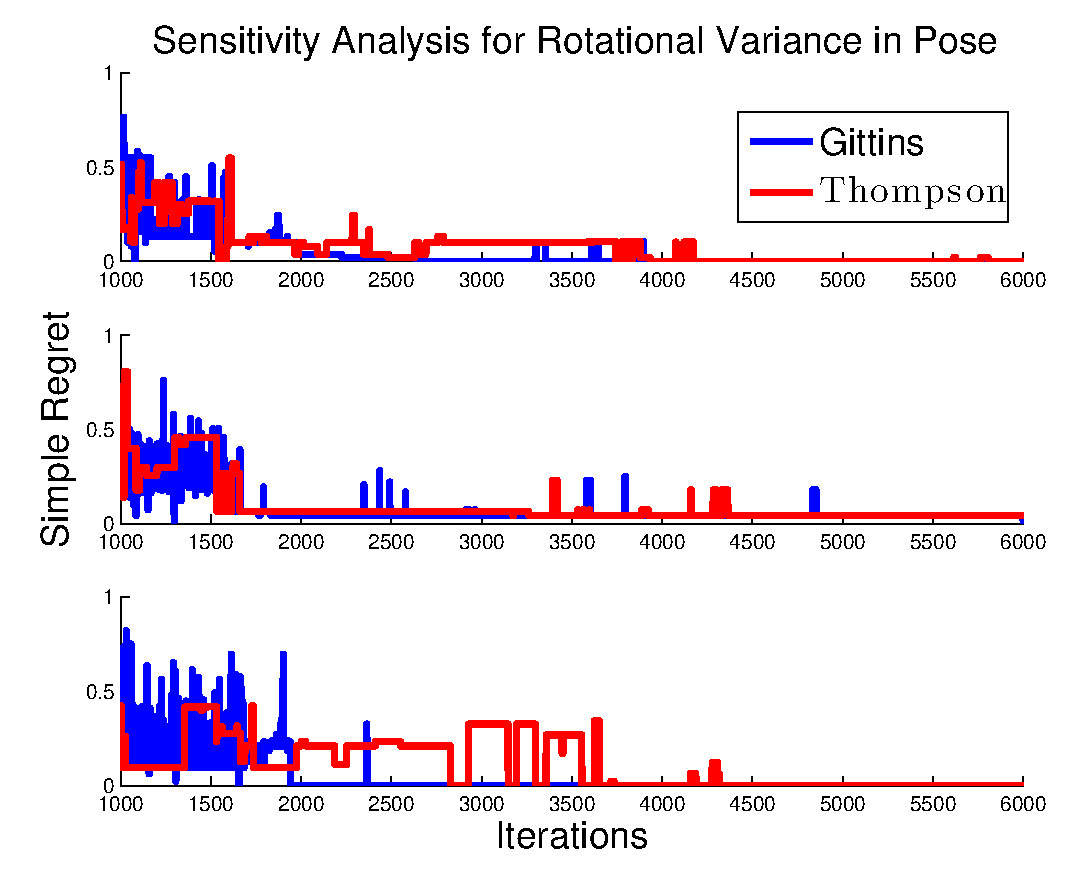
\includegraphics[width = 8cm, height = 10cm]{matlab_figures/sensitivity_rot.eps}
\caption{ \footnotesize Sensitivity Analysis for Thompson Sampling and the Gittens Index Method under coefficient of friction uncertainty $\sigma_{rot} = \lbrace 0.03,0.12, 0.24 \rbrace$ radians from top to bottom on a 40 x 40 unit workspace averaged over 10 shapes from the Brown Vision Lab Data set. The increase in noise has little effect on the convergence of the two algorithms in simple regret. \todo{Going to rerun with more shapes to be sure about this}}
\vspace*{-10pt}
\label{fig:rot_sens}
\end{figure}

\begin{figure*}%
    \centering
    \subfloat[lTop Grasps Shown for Shape 1]{{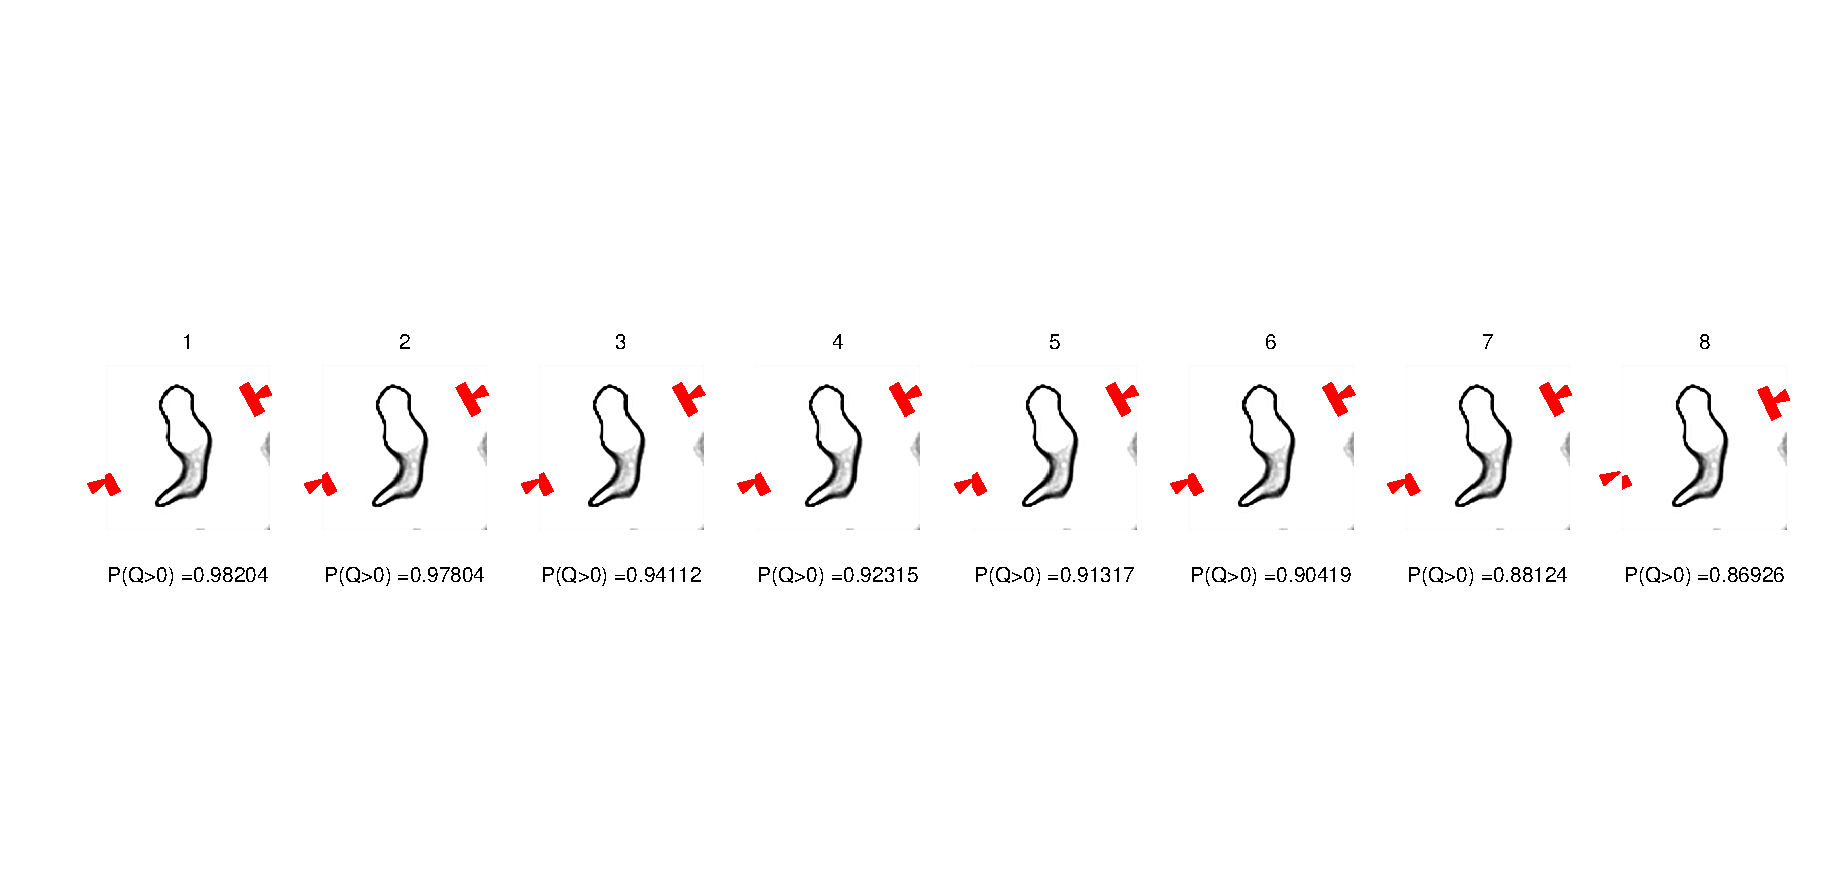
\includegraphics[width=16.5cm]{matlab_figures/rot_shapes_1.eps} }}%
    \qquad
    \subfloat[Top Grasps Shown for Shape 2]{{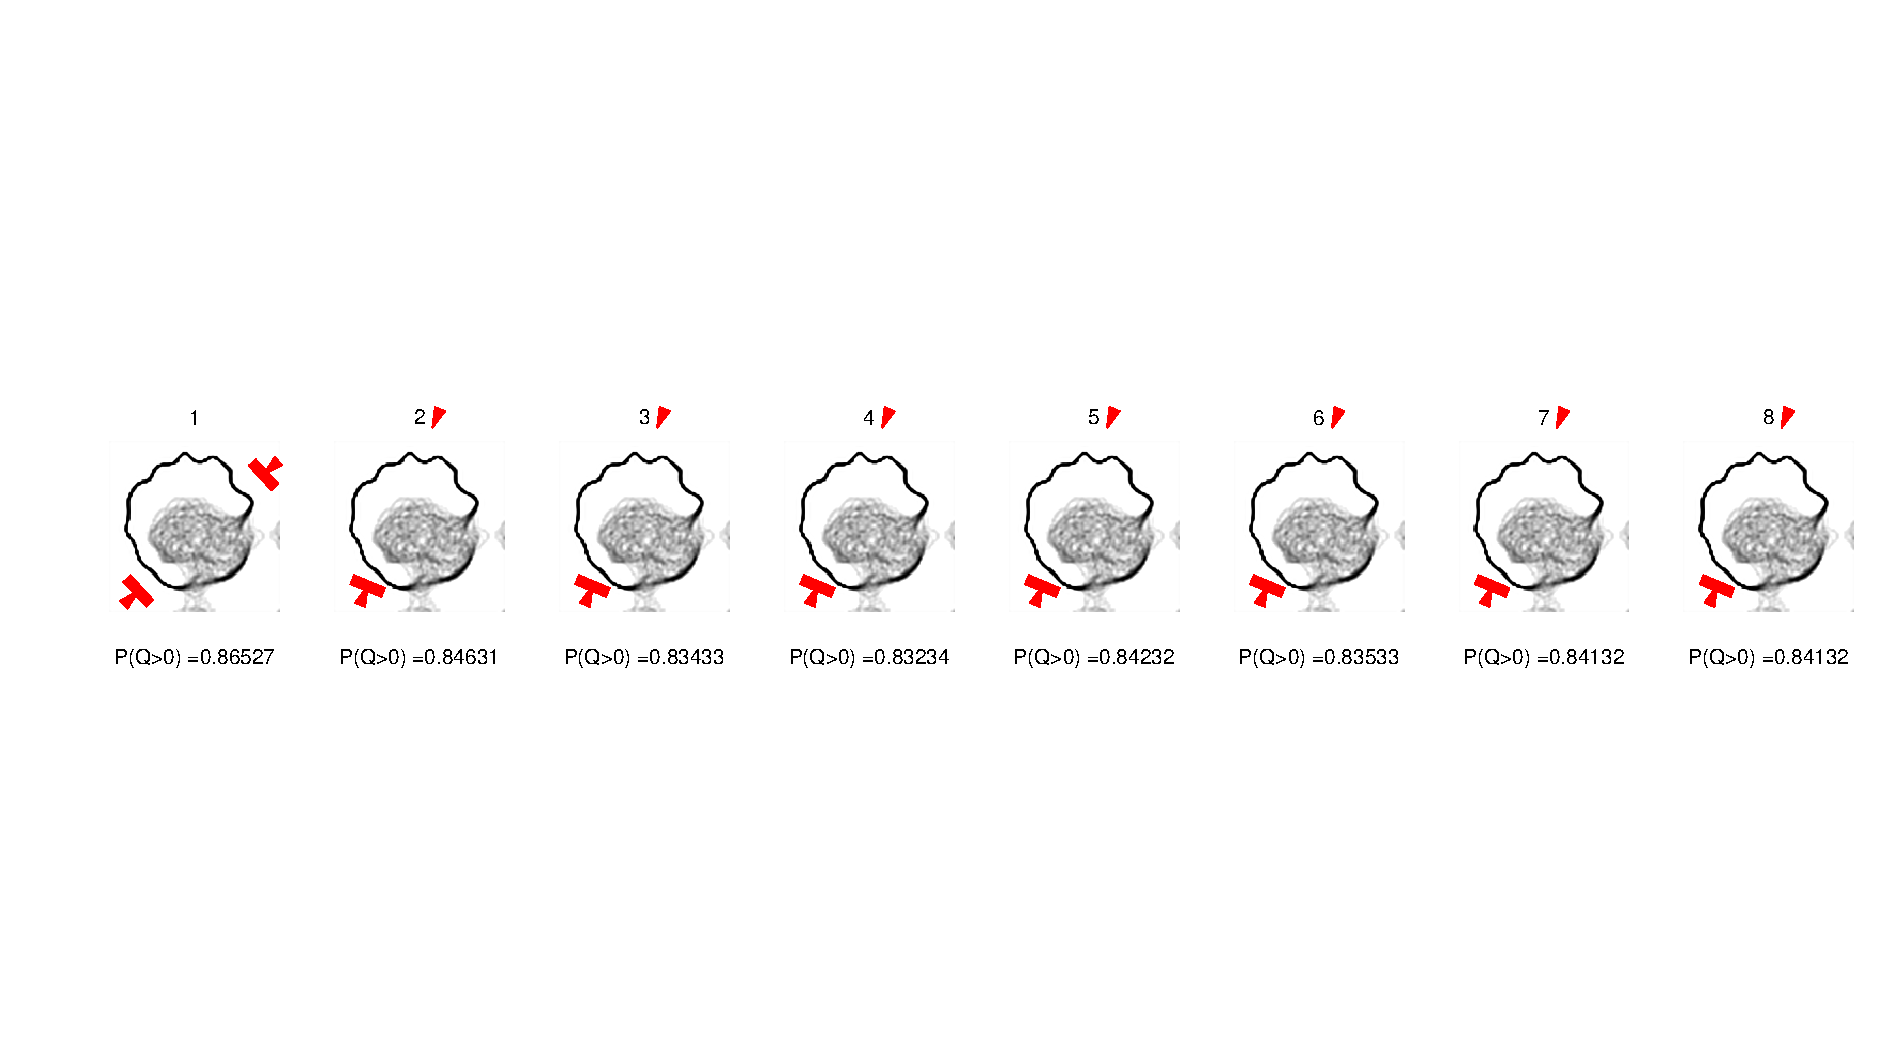
\includegraphics[width=16.5cm]{matlab_figures/rot_shapes_2.eps} }}%
    \caption{Two shapes shown from the Brown Visual Lab Dataset,from Left to Right the variance on rotation $\sigma_{rot}$ is increased $0.03$, $0.12$ to $0.24$ radians.  As you can see the overall variance increase effects the quality of the top grasp in the set of possible grasps. Furthermore for Shape 2, the grasp with low rotational variance is different than that for higher variance because the original grasp is more likely to touch the area of higher shape uncertainty when subjected to high variance in rotation. \todo{find better shapes in the brown dataset} }%
    \label{fig:rot_shapes}%
\end{figure*}


\begin{figure}[ht!]
\centering
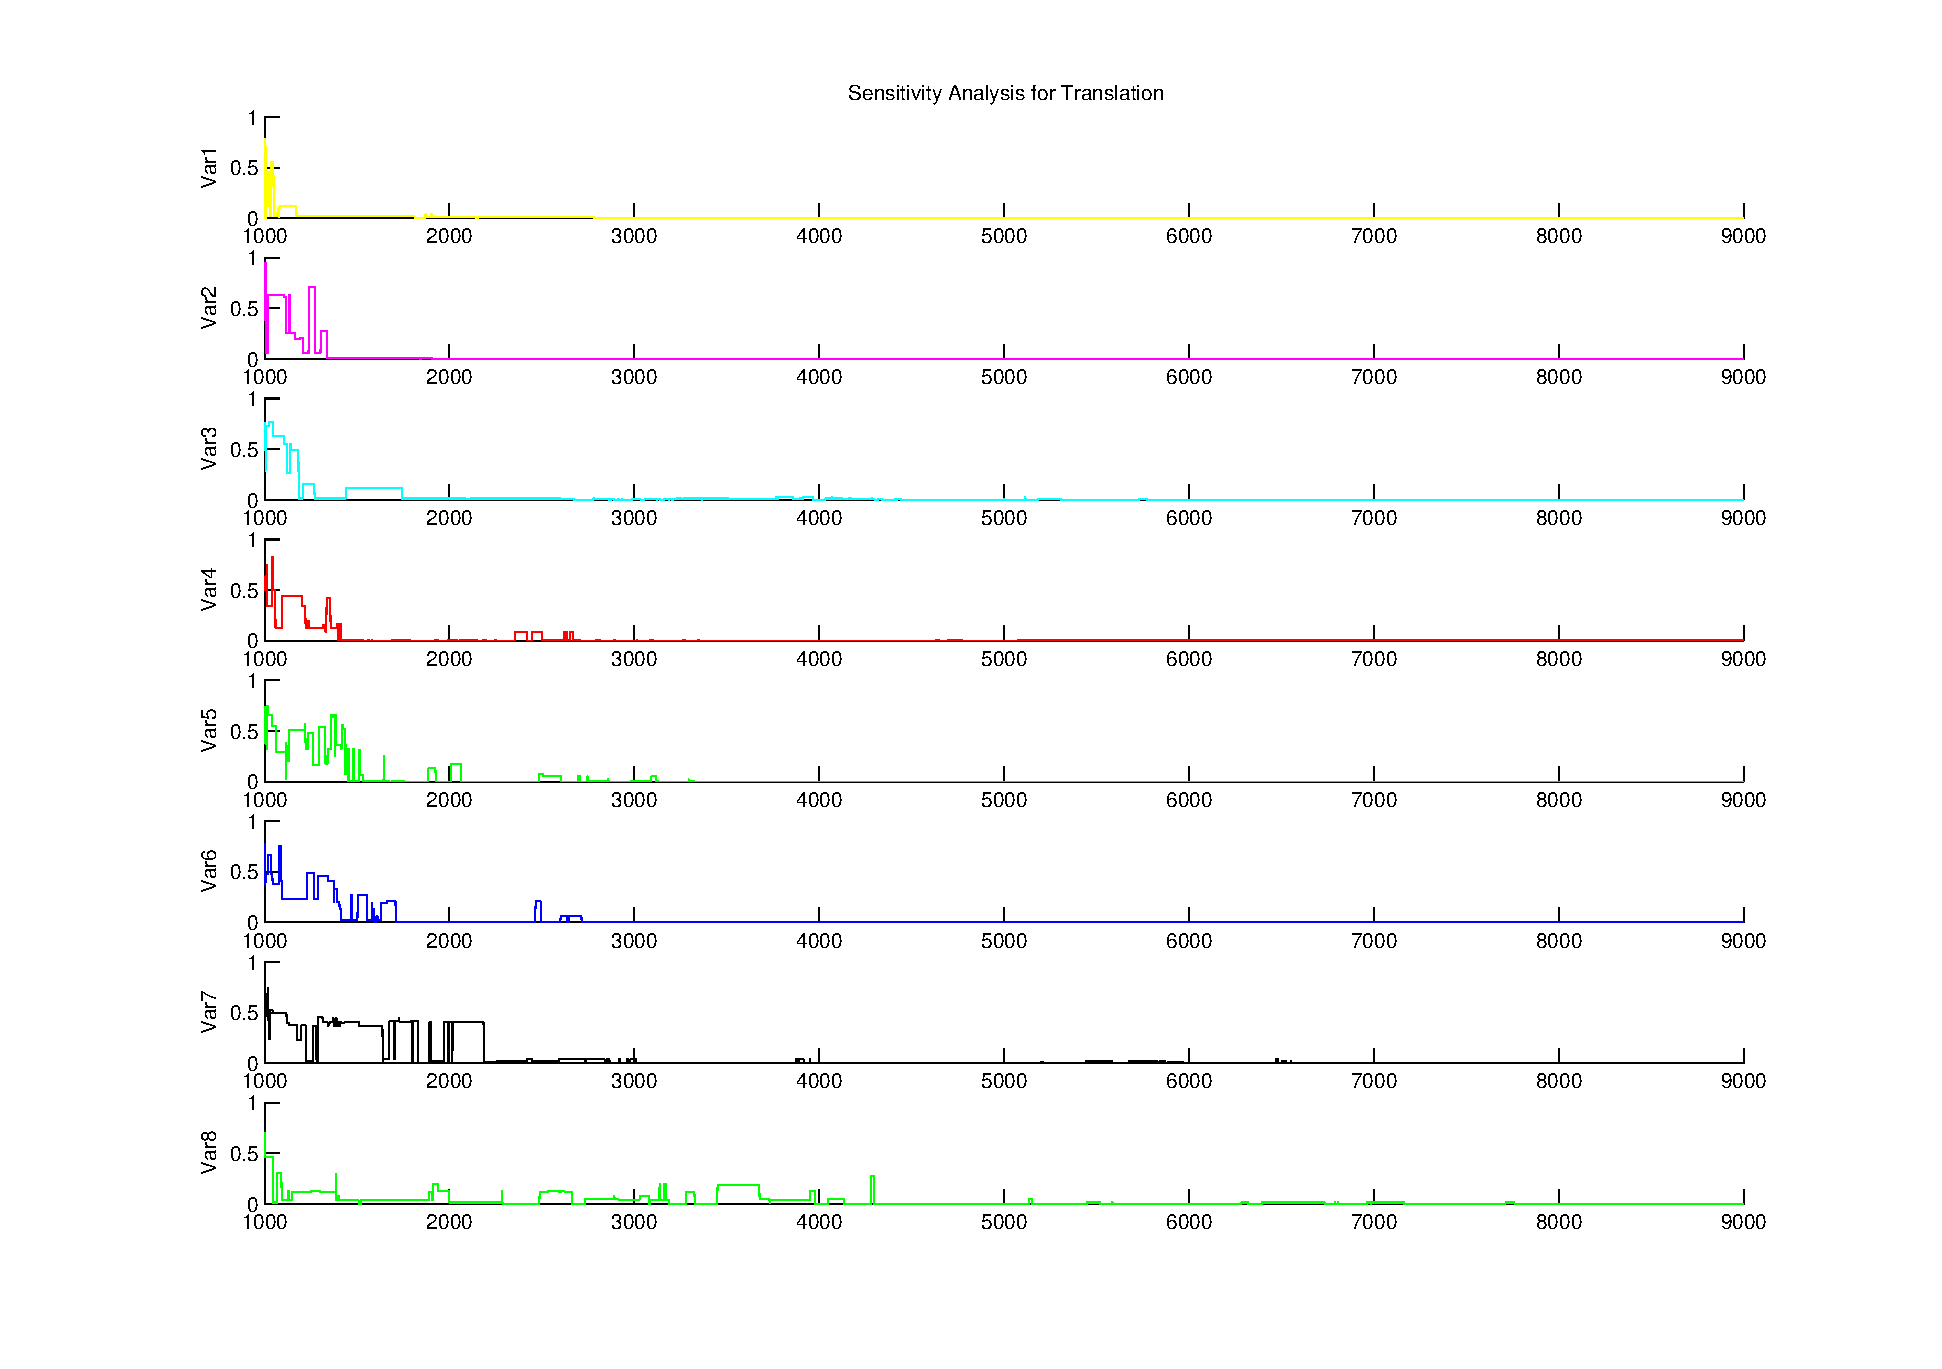
\includegraphics[width = 8cm, height = 10cm]{matlab_figures/sensitivity_trans.eps}
\caption{ \footnotesize Sensitivity Analysis for Thompson Sampling under translation uncertainty $\sigma_{trans} = \lbrace 3, 12, 24 \rbrace$ units from top to bottom on a 40 x 40 unit workspace.  As you can see the increase in noise effects performance, however the 5000 samples needed for Gittins to  converge at the the highest level of noise (which is a variance of over half the workspace) is much less that the samples needed for uniform allocation to converge in Fig. \ref{fig:simple_regret}}
\vspace*{-10pt}
\label{fig:trans_sens}
\end{figure}






\section{Limitations} 

Our budgeted multi-armed bandit approach appears promising, but we still do not know how well it will perform on 3D shapes and large scale grids. Future work will be building an efficient construction of GPIS to scale to 3D and test the bandit method there. 

The methods we showed (UCB, Thompson and Gittins) are guranteed to find the best grasp as the stopping time approaches infinity \cite{kaufmann2012bayesian,grawal2011analysis,weber1992gittins} but when do you terminate the algorithm is still an open question. Fixed confidence methods do exist that terminate when a certain confidence interval is reached \cite{maron1993hoeffding} \cite{mnih2008empirical}. However, a known problem is that if two grasps have very similar quality it could greatly increase the time for needed to reach the statistical confidence interval \cite{audibert2010best}. We proposed treating the BMAB as anytime algorithm and have demonstrated empirically that the grasps at a given stopping time are better than prior methods of Monte-Carlo sampling or the approach of Kehoe et al. However, this has a hyper parameter that has to be user-defined, which is not ideal.  

Another problem that was revealed in our analysis was that our current grasp metric, probability of force closure, is not dependent on the center of mass \cite{ferrari1992}. It only measure the probability that a grasp controller can resist any force provided it can exert an infinite force.  One can assume that the grasp controller on a robot hand is powerful enough to apply the proper resistance, but that assumption might be invalid in some applications. A similar metric that is still from Beta-Bernoulli and takes center of mass into account, would be ideal for both accurate grasp quality prediction under uncertainty and the utilization of MAB algorithms.  Recent work by Kim et al. developed a physics based simulator that could potentially achieve this goal \cite{kim2012physically}. 

\section{Conclusion}
Assessing grasp quality under  uncertainty is computationally expensive as it often requires repeated evaluations of the grasp metric over many random samples.
In this work, we proposed a multi-armed bandit approach to efficiently identify high-quality grasps under uncertainty in shape, pose, friction coeffiecient and motion. 
A key insight from our work is that uniformly allocating samples to grasps is inefficient, and
 we found that a MAB approach prioritizes evaluation of high-quality grasps while quickly pruning-out obviously poor grasps.
A pre-requisite for applying a bandit approach is to formulate a representation  of how uncertainty affects grasp parameters and thus grasp quality.
We purpose treating this as a graphical model and use model the parameters as stochastic noise. Our choice of distributions though is not the focus of the paper. The MAB algorithm is applicable in any context of bounded reward distributions and all the theoretical results we mentioned will transfer to the Beta-Bernoulli case, or the estimation of probability of force closure. 

Our anytime BMAB approach is guaranteed to find the best grasp in a given proposal set in the limit of an infinite time and has empirically been shown to outperform the methods of prior work Monte-Carlo and the method purposed by Kehoe et al. \cite{kehoe2012estimating}. 



\section{Future Work}
Our results are promising and they suggest many avenues of future work. By utilizing the BMAB model, we can encode uncertainty in the grasp parameters and then leverage the existing algorithms to efficiently find the best grasp. 

In principle, our method can be applied to other representations of shape uncertainty such as perturbations on polygonal vertices \cite{kehoe2012estimating} or splines \cite{christopoulos2007handling}.
It can further be applied to other grasp quality metrics or simulation based evaluation methods \cite{73}. 

Future work will also consider applying BMAB approach to grasp planners like GraspIt! \cite{miller2004graspit} to see if our method can handle uncertainty while working under the time constraints needed for most real time applications. While our results are promising, it remains to be seen how well it deals with the increased complexity of 3D models over 2D models and larger scale experiments. However, the BMAB model has a large amount of literature to draw from as we encounter new and more challenging problems \cite{bergemann2006bandit}.

\bibliographystyle{IEEEtranS}
\bibliography{references}


\appendix[Gaussian Process Implicit Surface for Representing Shape Uncertainty]
 \label{sec:Appendix}
 In order to solve our problem definition, we must estimate $P(Q(\Gamma)>0)$ for a given grasp . We will first discuss how the GPIS is constructed, then which grasp metric $Q$ we chose and lastly proceed into evaluating $P(Q(\Gamma)>0)$ efficiently. 


\subsection{Gaussian Process (GP) Background}\label{sec:GP}
We refer the reader to \cite{mahler2015opt} for a more detailed explanation of the GP construction, which we summarize here.  Given the training data $\mD = \{\mX, \by\}$ and covariance function $k(\cdot,\cdot)$, the posterior density $p(sd_*|\bx_*,\mD)$, or the distribution on signed distance field, at a test point $\bx_{*}$ is shown to be \cite{rasmussen2010gaussian}:
\begin{align*}
	p(sd_*|\bx_*,\mD) &\sim \mN\big(\mu(\bx_*), \Sigma(\bx_*)\big) \\
	\mu(\bx_*) &= k(\mX,\bx_*)^{\intercal}(K + \sigma^2I)^{-1}\by \\
	\Sigma(\bx_*) &= k(\bx_*,\bx_*)-k(\mX,\bx_*)^{\intercal}(K+\sigma^2I)^{-1}k(\mX,\bx_*)\big) 
\end{align*}
where $K \in \mathbb{R}^{l \times l}$ is a matrix with entries $K_{ij} = k(\bx_i,\bx_j)$ and $k(\mX,\bx_*) = [k(\bx_1,\bx_*),\ldots,k(\bx_l,\bx_*)]^{\intercal}$. 
This derivation can also be used to predict the mean and variance of the function gradient by extending the kernel matrices using the identities \cite{solak2003derivative}:

\vspace{-2ex}
\begin{align}
	\text{cov}\left(sd(\bx_i), sd(\bx_j) \right) &=  k(\bx_i, \bx_j) \\
	\text{cov}\left(\frac{\partial sd (\bx_i)}{\partial x_k}, sd(\bx_j) \right) &= \frac{\partial}{\partial x_k} k(\bx_i, \bx_j) \label{eq:mean_gradient}\\
	\text{cov}\left(\frac{\partial sd (\bx_i)}{\partial x_k}, \frac{\partial sd (\bx_j)}{\partial x_l} \right) &= \frac{\partial^2}{\partial x_k \partial x_l} k(\bx_i, \bx_j)\label{eq:cov_gradient}
\end{align}


For our kernel choice we decided to use the square exponential kernel, similar to \cite{dragiev2011}. Other kernels relevant to GPIS are the thin-plate splines kernel and the Matern kernel \cite{williams2007}. 


We construct a GPIS by learning a Gaussian process to fit measurements of a signed distance field of an unknown object.  Precisely, $x_i \in \mathbb{R}^2$ in 2D and $x_i \in \mathbb{R}^3$ in 3D, and $y_i \in \mathbb{R}$ is a noisy signed distance measurement to the unknown object at $x_i$.



\subsection{Sampling Shape from GPIS Distribution }
To compute the above distribution we must draw samples from $p(\theta)$. In order to draw shape samples from a GPIS, one needs to sample from signed distance function, $sd$, over the joint on all points in the workspace $\mathcal{W}$ or $p(sd(\mathcal{W}))$. Since this is a GPIS, we know the following 

\vspace{-2ex}
\begin{align}\label{eq:joint_shape}
p(S) = p(sd(\mathcal{W})) \sim N(\mu(\mathcal{W}),\Sigma(\mathcal{W}))
\end{align}

Thus if the workspace is an $n \times n$ grid, the joint distribution is an  $n^2$ multi-variate Gaussian, due to $sd:\mathbb{R}^2 \rightarrow \mathbb{R}$.  Shape samples drawn from the distribution appear in Fig. \ref{fig:shape_samples}.


\begin{figure}[ht!]
\centering
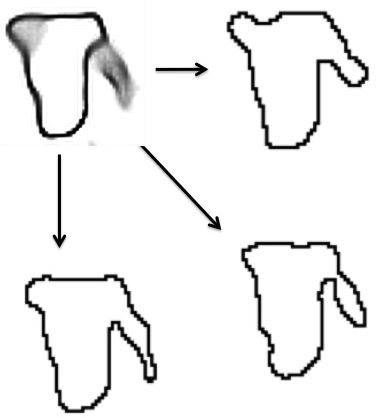
\includegraphics[width = 7.5cm, height= 6cm ]{figures/Slide13.jpg}
\caption{Shape samples drawn from Eq. \ref{eq:joint_shape} on the object in the upper left corner. Given a shape sample we highlight the zero-crossing of the level set in black}
\vspace*{-10pt}
\label{fig:shape_samples}
\end{figure}

\subsection{Distribution on Surface Normals}\label{sec:normals} 
Using Eq. \ref{eq:mean_gradient} and Eq. \ref{eq:cov_gradient}, we can compute the mean of the gradient $ \mu_{\nabla}(x)$ and the covariance of the gradient $\Sigma_{\nabla}(x)$ respectively. Thus we can compute the distribution around the surface normal for a given point in $\mathcal{W}$. We can now write 

One interesting effect of this technique is that we can now marginalize out the line of action model and visual what the surface normal distribution is along a given line of action. To our knowledge this is the first attempt to visual surface normals along a grasp plan. Marginalization can be performed as follows:

\vspace{-2ex}
\begin{equation}
    p(\textbf{n}_i ) = \int_a^b   p\big(\textbf{n}_i = \textbf{v} | \textbf{c}_i = \gamma(t) \big)p\big(\textbf{c}_i = \gamma(t)\big) dt \label{eq:normal_dist}
\end{equation}

Grasp metrics such as  Ferrari-Canny require $\textbf{n}_i$ be normalized, or, equivalently, a member of the sphere $\mathcal{S}^{d-1}$ \cite{ferrari1992}. To account for this we densely sample from the  distribution $p \big(\textbf{n}_i ) \big)$  and project onto $\mathcal{S}^{d-1}$.  In Fig.\ref{fig:GraspDist}, we visualize the distribution on $\textbf{n}_i$ calculated for a given GPIS and approach line of action.


\subsection{Expected Center of Mass}\label{sec:mass} 

We recall the quantity $P(sd(x) < 0) = \int_{-\infty}^{0} p(sd(x) =  s \ | \ \mu(x),\Sigma(x)) ds$ is equal to the probability that $x$ is interior to the surface under the current observations.
We assume that the object has uniform mass density and then $P(sd(x) < 0)$ is the expected mass density at $x$.
Then we can find the expected center of mass as:

\label{eq:mass}
\begin{equation}
  \bar{z} 
  =
  \frac
    {\int_{\mathcal{W}}x P(sd(x)<0) dx}
    {\int_{\mathcal{W}}  P(sd(x)<0) dx}
\end{equation}

which can be approximated by sampling $\mathcal{W}$ in a grid and approximating the spatial integral by a sum. Since this operation involves the entire SDF, one would want to use a low resolution grid for computational efficiency. We show the computed density and calculated expected center of mass for a marker in Fig. \ref{fig:GPIS_MASS}.


\begin{figure}[ht!]
\centering
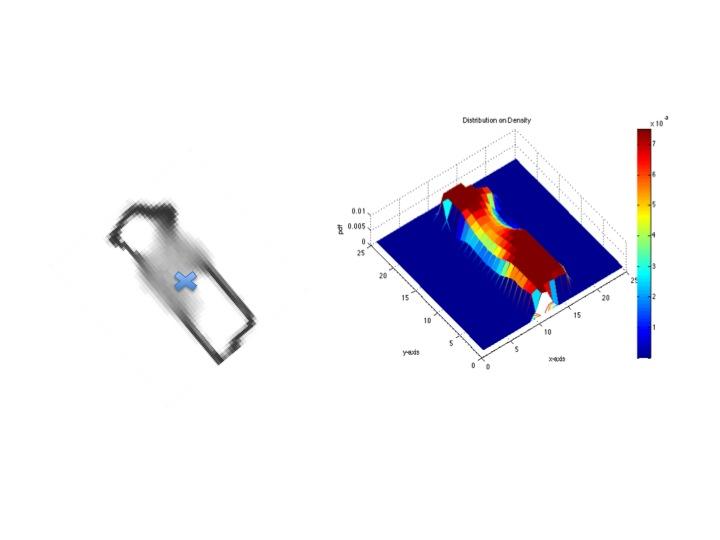
\includegraphics[scale = 0.3]{figures/Slide06.jpg}
\caption{ \footnotesize Left: A surface with GPIS construction and expected center of mass (black X)
Right: The distribution on the density of each point assuming uniform density}
\vspace*{-10pt}
\label{fig:GPIS_MASS}
\end{figure}








\end{document}
